%%% On-going present
%%
%% Beginning of file 'sample.tex'
%%
%% Modified 2005 December 5
%%
%% This is a sample manuscript marked up using the
%% AASTeX v5.x LaTeX 2e macros.

%% The first piece of markup in an AASTeX v5.x document
%% is the \documentclass command. LaTeX will ignore
%% any data that comes before this command.

%% The command below calls the preprint style
%% which will produce a one-column, single-spaced document.
%% Examples of commands for other substyles follow. Use
%% whichever is most appropriate for your purposes.
%%
%%\documentclass[12pt,preprint]{aastex}

%% manuscript produces a one-column, double-spaced document:

%%\documentclass[manuscript]{aastex}

%% preprint2 produces a double-column, single-spaced document:

 %\documentclass[preprint2]{aastex}
%\documentclass[preprint2]{aastex}
%\documentclass[manuscript]{aastex}
\documentclass[iop]{emulateapj}
\renewcommand{\baselinestretch}{0.95}
%% Sometimes a paper's abstract is too long to fit on the
%% title page in preprint2 mode. When that is the case,
%% use the longabstract style option.

%% \documentclass[preprint2,longabstract]{aastex}

%% If you want to create your own macros, you can do so
%% using \newcommand. Your macros should appear before
%% the \begin{document} command.
%%
%% If you are submitting to a journal that translates manuscripts
%% into SGML, you need to follow certain guidelines when preparing
%% your macros. See the AASTeX v5.x Author Guide
%% for information.

\usepackage{enumitem} 

\newcommand{\hMsun}{{\ifmmode{h^{-1}{\rm
        {M_{\odot}}}}\else{$h^{-1}{\rm{M_{\odot}}}$~}\fi}} 
\newcommand{\hMpc}{{\ifmmode{h^{-1}{\rm Mpc}}\else{$h^{-1}$Mpc }\fi}}
\def\be{\begin{equation}}
\def\ee{\end{equation}}
\def\ba{\begin{eqnarray}}
\def\ea{\end{eqnarray}}


%% You can insert a short comment on the title page using the command below.

%\slugcomment{Not to appear in Nonlearned J., 45.}

%% If you wish, you may supply running head information, although
%% this information may be modified by the editorial offices.
%% The left head contains a list of authors,
%% usually a maximum of three (otherwise use et al.).  The right
%% head is a modified title of up to roughly 44 characters.
%% Running heads will not print in the manuscript style.

%\title[]
%{}

\shorttitle{Reshift Dependent Volume effect}
\shortauthors{X.-D. Li, C. Park, C.G. Sabiu, H. Park, D.H. Weinberg, J. Kim, S.E. Hong}

%% This is the end of the preamble.  Indicate the beginning of the
%% paper itself with \begin{document}.

\begin{document}

%% LaTeX will automatically break titles if they run longer than
%% one line. However, you may use \\ to force a line break if
%% you desire.

\title{Cosmological constraints from the redshift dependence of %geometric deformation
the galaxy angular 2-point correlation function}


%\author{Xiao-Dong~Li\altaffilmark{1}, Changbom~Park\altaffilmark{1}, J.~E.~Forero-Romero\altaffilmark{2} and Juhan Kim%\altaffilmark{3}}
%\affil{\altaffilmark{1}School of Physics, Korea Institute for Advanced Study, Heogiro 85, Seoul 130-722, Korea }
%\affil{\altaffilmark{2}Departamento de F\'{i}sica, Universidad de los Andes, Cra. 1 No. 18A-10, Edificio Ip, Bogot\'a, %Colombia}
%\affil{\altaffilmark{3}Center for Advanced Computation, Korea Institute for Advanced Study, 85 Hoegi-ro, Dongdaemun-%gu, Seoul 130-722, Korea }
%\affil{\it (xiaodongli@kias.re.kr, cbp@kias.re.kr, je.forero@uniandes.edu.co, kjhan@kias.re.kr)}

%\author[Xiao-Dong~Li, Changbom~Park, Cristiano G. Sabiu, Juhan Kim and Sungwook E. Hong]
%{ Xiao-Dong Li$^{1,\dagger}$, Changbom Park$^{1}$, Cristiano G. Sabiu$^{2}$, Juhan Kim$^{3,1,\star}$, Sungwook E. Hong$^{1}$\\
%$^1$School of Physics, Korea Institute for Advanced Study, 85 Heogi-ro, Dongdaemun-gu, Seoul 130-722, Korea\\
%$^2$Korea Astronomy and Space Science Institute, 776, Daedeokdae-ro, Yuseong-gu, Daejeon, 305-348, Korea\\
%$^3$Center for Advanced Computation, Korea Institute for Advanced Study, 85 Hoegi-ro, Dongdaemun-gu, Seoul 130-722, Korea\\
%$^{\dagger}$xiaodongli@kias.re.kr\\
%$\star$Corresponding Author: ***@kasi.re.kr}

\author{Xiao-Dong Li, }
\affil{School of Physics, Korea Institute for Advanced Study, 85 Heogiro, Dongdaemun-gu, Seoul 130-722, Korea}
\author{Cheng Cheng, }
\affil{Kavli Institute for Theoretical Physics China, Institute of Theoretical Physics, Chinese Academy of Sciences, Zhong Guan Cun Street 55\#, Beijing, 100190, P.R. China}
\affil{University of Chinese Academy of Sciences, P.R. China}
\author{Changbom Park,}
\affil{School of Physics, Korea Institute for Advanced Study, 85 Heogiro, Dongdaemun-gu, Seoul 130-722, Korea}
\author{Cristiano G. Sabiu, Hyunbae Park,}
\affil{Korea Astronomy and Space Science Institute, Daejeon 305-348, Korea}
%\author{David H. Weinberg,}
%\affil{Department of Astronomy and CCAPP, The Ohio State University, 140 West 18th Avenue, Columbus, OH 43210, USA}
%\author{Donald P. Schneider,}
%\affil{Department of Astronomy and Astrophysics, The Pennsylvania State University, 
%University Park, PA 16802 }
%\affil{Institute for Gravitation and the Cosmos, The Pennsylvania State University, 
%University Park, PA 16802 }
\author{Juhan Kim\altaffilmark{1},}
\affil{Center for Advanced Computation, Korea Institute for Advanced Study, 85 Hoegi-ro, Dongdaemun-gu, Seoul 130-722, Korea}
\affil{School of Physics, Korea Institute for Advanced Study, 85 Heogiro, Dongdaemun-gu, Seoul 130-722, Korea}
\and
\author{Sungwook E. Hong}
\affil{School of Physics, Korea Institute for Advanced Study, 85 Heogiro, Dongdaemun-gu, Seoul 130-722, Korea}

%\altaffiltext{1}{xiaodongli@kias.re.kr}
%\altaffiltext{2}{cbp@kias.re.kr}
%\altaffiltext{3}{csabiu@kasi.re.kr}
%\altaffiltext{4}{\bf Hyunbae: your email}
\altaffiltext{1}{Corresponding Author: kjhan@kias.re.kr}

% \email{xiaodongli@kias.re.kr}
% \email{cbp@kias.re.kr}
% \email{je.forero@uniandes.edu.co}



% \author{S. Djorgovski\altaffilmark{1,2,3} and Ivan R. King\altaffilmark{1}}
% \affil{Astronomy Department, University of California,
%     Berkeley, CA 94720}
%
% \author{C. D. Biemesderfer\altaffilmark{4,5}}
% \affil{National Optical Astronomy Observatories, Tucson, AZ 85719}
% \email{aastex-help@aas.org}
%
% \and
%
% \author{R. J. Hanisch\altaffilmark{5}}
% \affil{Space Telescope Science Institute, Baltimore, MD 21218}
%
% %% Notice that each of these authors has alternate affiliations, which
% %% are identified by the \altaffilmark after each name.  Specify alternate
% %% affiliation information with \altaffiltext, with one command per each
% %% affiliation.
%
% \altaffiltext{1}{Visiting Astronomer, Cerro Tololo Inter-American Observatory.
% CTIO is operated by AURA, Inc.\ under contract to the National Science
% Foundation.}
% \altaffiltext{2}{Society of Fellows, Harvard University.}
% \altaffiltext{3}{present address: Center for Astrophysics,
%     60 Garden Street, Cambridge, MA 02138}
% \altaffiltext{4}{Visiting Programmer, Space Telescope Science Institute}
% \altaffiltext{5}{Patron, Alonso's Bar and Grill}

%% Mark off your abstract in the ``abstract'' environment. In the manuscript
%% style, abstract will output a Received/Accepted line after the
%% title and affiliation information. No date will appear since the author
%% does not have this information. The dates will be filled in by the
%% editorial office after submission.

\begin{abstract}
We use the shape of galaxy 2-point correlation function to measure the redshift dependence cosmology volume effect.
...
\end{abstract}

%% Keywords should appear after the \end{abstract} command. The uncommented
%% example has been keyed in ApJ style. See the instructions to authors
%% for the journal to which you are submitting your paper to determine
%% what keyword punctuation is appropriate.

\keywords{large-scale structure of Universe --- dark energy --- cosmological parameters}

%% From the front matter, we move on to the body of the paper.
%% In the first two sections, notice the use of the natbib \citep
%% and \citet commands to identify citations.  The citations are
%% tied to the reference list via symbolic KEYs. The KEY corresponds
%% to the KEY in the \bibitem in the reference list below. We have
%% chosen the first three characters of the first author's name plus
%% the last two numeral of the year of publication as our KEY for
%% each reference.


%% Authors who wish to have the most important objects in their paper
%% linked in the electronic edition to a data center may do so by tagging
%% their objects with \objectname{} or \object{}.  Each macro takes the
%% object name as its required argument. The optional, square-bracket
%% argument should be used in cases where the data center identification
%% differs from what is to be printed in the paper.  The text appearing
%% in curly braces is what will appear in print in the published paper.
%% If the object name is recognized by the data centers, it will be linked
%% in the electronic edition to the object data available at the data centers
%%
%% Note that for sources with brackets in their names, e.g. [WEG2004] 14h-090,
%% the brackets must be escaped with backslashes when used in the first
%% square-bracket argument, for instance, \object[\[WEG2004\] 14h-090]{90}).
%%  Otherwise, LaTeX will issue an error.

\section{Introduction}

Dark energy ... Large scale structure...

2pCF is a good statistic... blahblah
In 2d xi(s,mu) ...
In *** we used the redshift dependence of 2pCF to probe the volume and AP effect...
The method is applied to BOSS data in *** and obtain tight constraint...

In *** we further propose to use the shape of xi(s) to probe the volume effect...
Stretch or compression shifts the clustering properties in some particular scale to larger or smaller scales...
The shape of measured xi(s) is thus stretched or compressed.

The outline of this paper is as follows. 

This paper is organized as follows...
The outline of this paper proceeds as follows. 
In \S 2 we briefly review the nature and consequences of the AP effect and volume changes when performing coordinate transforms in a cosmological context. 
In \S 3 we describe the N-body simulations and mock galaxy catalogues that are used to test our methodology.
In \S 4, we describe our new analysis method for quantifying the redshift dependence of volume effect.
We conclude in \S 5.


\section{Geometric deformation when }
\label{sec:Voleffect}

\begin{figure*}
   \centering{
   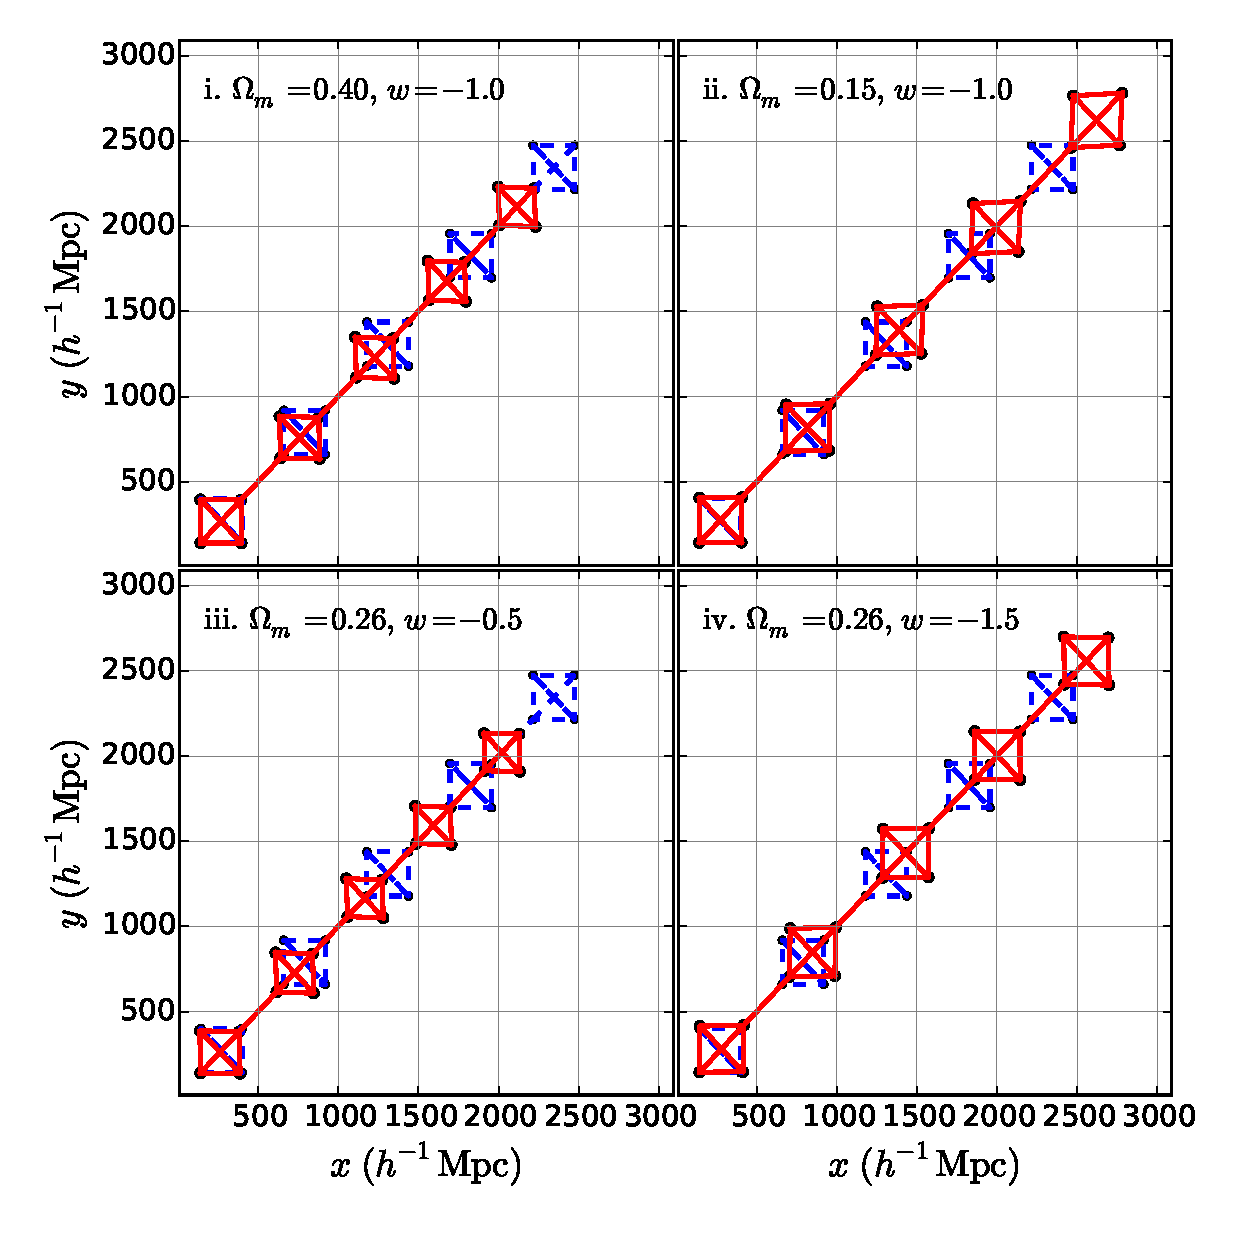
\includegraphics[height=8cm]{fig1_a.eps}
   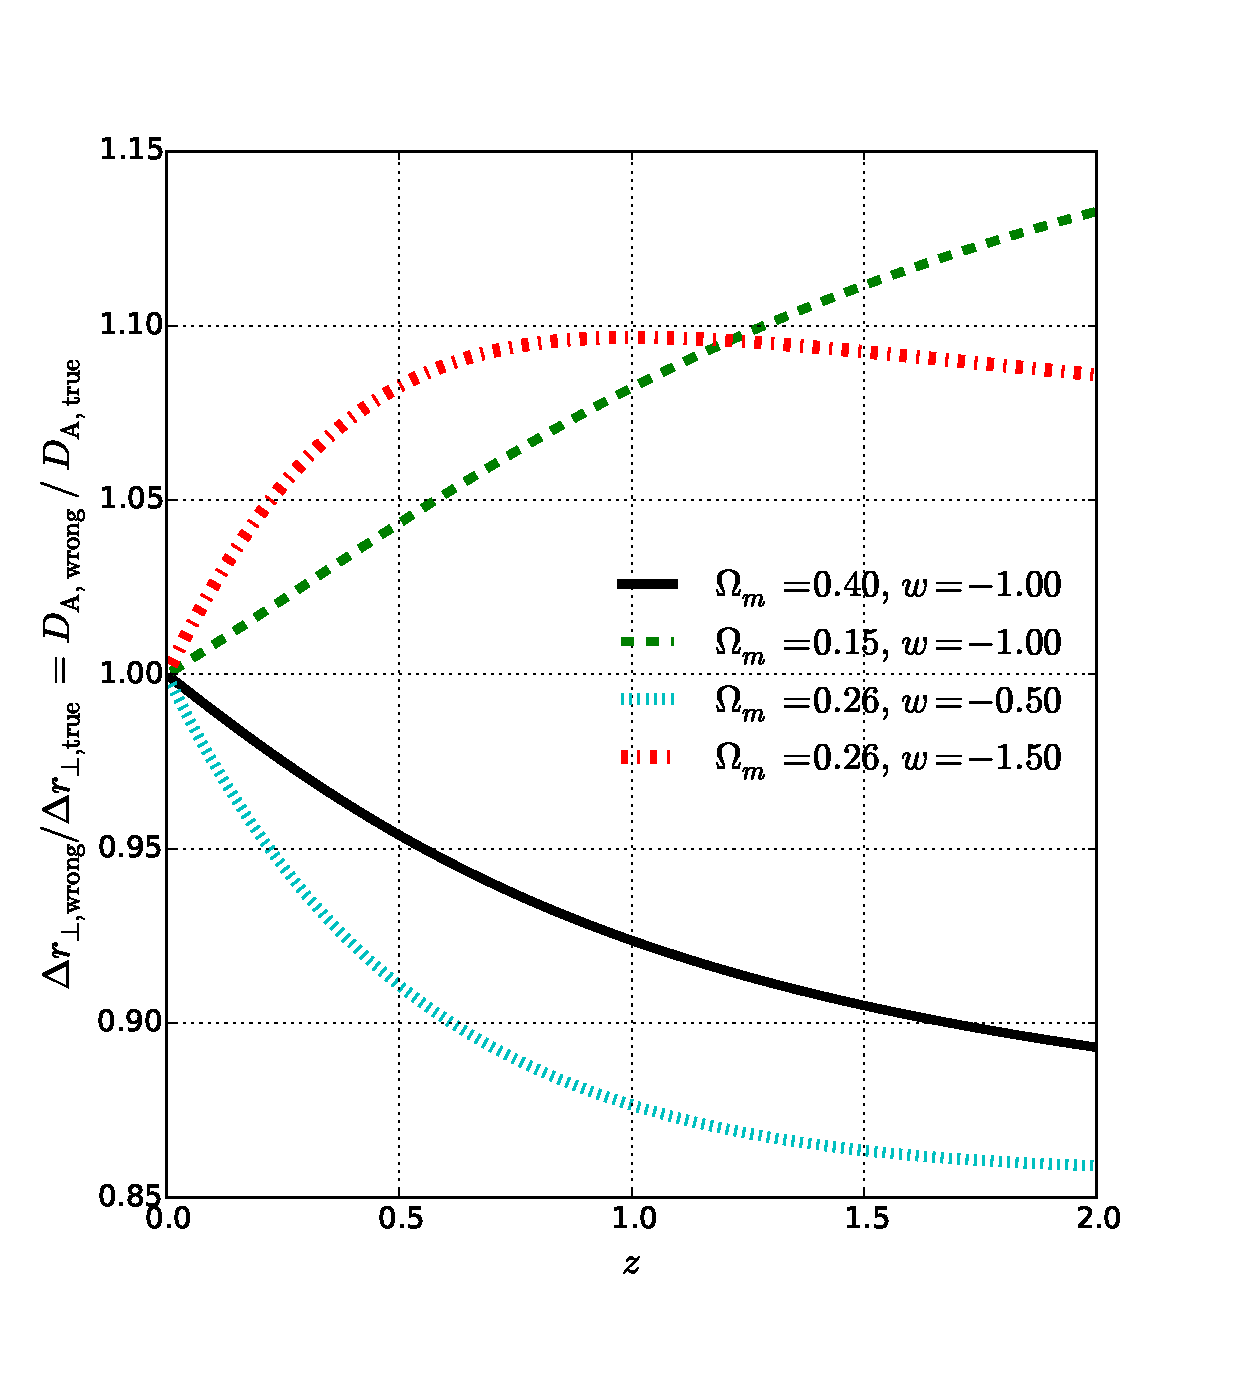
\includegraphics[height=8.5cm]{fig1_b.eps}
   }
   \caption{\label{fig_xyquan}
   %Apparent distortion of objects in four wrongly assumed cosmologies, assuming a true cosmology of .
   The scaling in four wrongly assumed cosmologies ..., % $\Omega_m=0.41$, $w=-1.3$ and $\Omega_m=0.11$, $w=-0.7$, 
   assuming a true cosmology of $\Omega_m=0.26$, $w=-1$.
   Left panel shows a series objects distributes as five perfect squares, measured by an observer located at the origin.
   Their true positions and shapes are plotted in blue dashed lines.
   The observer measures the redshifts of these objects, adopts the wrong cosmologies to compute the distance,
   and obtains wrong results (the red solid lines).
   %The red solid lines show their positions and shapes when the wrong cosmologies 
   % are assumed to compute distance from measured redshift.
   %The misestimation of angular diameter distance lead to wrong 
   Right panel shows the misestimation of angular diameter distance when the wrong cosmologies are adopted.
   %In our mock surveys we split the samples at $z=0.3$, 0.6, 0.9 and 1.2, as marked by the vertical lines.
   %measured by an observer located at the origin.
   %For reference, blue dashed squares show their shapes and positions in the true cosmology.
   }
   % Need a better plot to show angular size variation!!!
\end{figure*}

%Considering we are Let us consider an object in the universe with certain size and shape.
%Its observed redshift span $\Delta z$ and angular size $\Delta \theta$ are related with the comoving sizes by
In this section we briefly introduce the scaling effect in wrongly assumed cosmologies.
A more detailed description has been provided in \cite{Li2014,Li2015,Li2016}.

Suppose that we are probing the shape of some objects in the Universe.
We measure its redshift span $\Delta z$ and angular size $\Delta \theta$,
then compute its sizes in the radial and transverse directions from the relations of 
\begin{equation}\label{eq:distance}
\Delta r_{\parallel} = \frac{c}{H(z)}\Delta z,\ \ \Delta r_{\bot}=(1+z)D_A(z)\Delta \theta,
\end{equation}
where $H$ is the Hubble parameter, $D_A$ is the angular diameter distance.
In the particular case of a flat universe with constant dark energy EoS, they take the forms of
\begin{eqnarray}\label{eq:HDA}
& &H(z) = H_0\sqrt{\Omega_ma^{-3}+(1-\Omega_m)a^{-3(1+w)}},\nonumber\\
& &D_A(z) = \frac{1}{1+z}r(z)=\frac{1}{1+z}\int_0^z \frac{dz^\prime}{H(z^\prime)},
\end{eqnarray}
where $a=1/(1+z)$ is the cosmic scale factor,
$H_0$ is the present value of Hubble parameter and $r(z)$ is the comoving distance.

In case we adopted a wrong set of cosmological parameters in Equation (\ref{eq:distance},\ref{eq:HDA}),
the inferred $\Delta r_{\parallel}$ and $\Delta r_{\bot}$ are wrong,
resulting in distorted shape (AP effect) and wrongly estimated volume (volume effect).
These effects have been discussed in \cite{Li2014,Li2015,Li2016}.
This paper we focus on the misestimation of $\Delta r_{\bot}$,%scaling of angular size,
which can be described by the following quantities
\begin{equation}\label{eq:DA}
 %{\rm Degree\ of\ volume\ magnification \equiv}
 %{\rm rat}_{\rm volume\ mag}\equiv
 \alpha_{\bot} \equiv \frac{\Delta r_{\bot, \rm wrong}}{\Delta r_{\bot, \rm true}}
 = \frac{D_{A, \rm wrong}}{D_{A, \rm true}},
\end{equation}
where ``true'' and ``wrong'' denote the values of $D_A$ in the true cosmology and wrongly assumed cosmology.

The effects due to wrongly assumed cosmological parameters are shown in the upper panel of Figure \ref{fig_xyquan}.
Suppose that the true cosmology is a flat $\Lambda$CDM with present density parameter $\Omega_m=0.26$
and standard dark energy EoS $w=-1$.
If we were to distribute a series of perfect squares at various distances from 500 Mpc/h to 3\,000 Mpc/h,
and an observer located at the origin were to measure their redshifts and compute their positions and shapes 
using redshift-distance relations of four incorrect cosmologies
\begin{eqnarray}
 & &{\rm (i)}.\ \Omega_m=0.40,\ w=-1.0, \nonumber \\ 
 & &{\rm (ii)}.\ \Omega_m=0.15,\ w=-1.0, \nonumber\\ \noindent
 & &{\rm (iii)}.\ \Omega_m=0.26,\ w=-0.5,\nonumber\\ \noindent
 & &{\rm (iv)}.\ \Omega_m=0.26,\ w=-1.5, \nonumber \noindent
\end{eqnarray}
the shapes of the squares appear distorted (AP effect),
and their volumes are changed (volume effect).
In the cosmological models in model (i,iii) we see a compression of size (in both angular and LOS direction)
and the degree of compression increases with increasing distance,
while in models (ii,iv) we see stretch of size whose degree also evolves with redshift.
Thus, when wrong cosmological parameters are adopted,
the apparent size of objects are distorted, and the magnitude of distortion also varies with redshift.

In this paper we will use the galaxy angular 2pCF to probe the redshift dependence of the distortion in angular direction.
In the right panel of Figure \ref{fig_xyquan} we plot the redshift dependence of the change in angular size, 
${\Delta r_{\bot, \rm wrong}}/{\Delta r_{\bot, \rm true}}$, in the four wrong cosmologies.
In all cosmologies, there is clear evolution of ${\Delta r_{\bot, \rm wrong}}/{\Delta r_{\bot, \rm true}}$ 
in the redshift range $0<z<2$.
E.g., when use the quintessence cosmology 
$\Omega_m=0.26,\ w=-0.5$ to infer the postions of objects,
the angular size is underestimated by 
%12.5\%, 17.7\%, 20.1\%, 21.3\%
8.9\%, 12.3\%, 13.6\%, 14.1\% 
at $z=0.5,1,1.5,2$.




\section{The Simulation Data}\label{sec:data}

We test the method on the Horizon Run 4  (HR4) simulation \citep{hr4}.
HR4 used $N=6300^3$ particles in a box size of $L={3150}$ $h^{-1}$Mpc.  
It adopted the second order Lagrangian perturbation theory (2LPT) initial conditions at $z_{i}=100$
and a WMAP5 cosmology $(\Omega_{b},\Omega_{m},\Omega_\Lambda,h,\sigma_8,n_s)$  = (0.044, 0.26, 0.74, 0.72, 0.79, 0.96) \citep[]{komatsu 2011}.
The particle mass is $\simeq m_{p} \simeq 9.02 \times 10^9 \hMsun$.
%This starting redshift, combined  with 2LPT initial conditions, ensures an accurate mass function and power spectrum \citep{2014NewA...30...79L}. 

Mock galaxy samples are produced from the simulation based on a modified one-to-one correspondence scheme \citep{hong2016}. 
The most bound member particles (MBPs) of simulated halos are adopted as the tracer of galaxies,
and the merger timescale is computed to get the lifetime of merged halos.
Merger trees of simulated halos are constructed by tracking their MBPs from $z = 12$ to 0.
When a merger event occurs, we adopt the formular of \cite{jiang2008} to calculate the merger timescale 
and determine when a satellite galaxy is completely disrupted.
%We modeled the position and the velocity of a galaxy from the position and velocity of its corresponding MBP.
%By using the abundance matching, 
%we modeled the luminosity of a central/isolated galaxies from their current mass
%and of satellite galaxies from their mass at the time of infall.

\cite{hong2016} compared the 2pCF of the SDSS DR7 volume-limited galaxy sample \citep{zehavi2011} and the HR4 $z=0$ mock galaxies.
%When a typical subhalo-galaxy correspondence scheme is applied, 
%the 2pCF from our simulation is smaller than the observation and does not show a proper Finger-of-God (FOG) feature in our simulation resolution. 
%We found that %the %2pCF of our galaxy sample agrees well with the observation.
The mock galaxies shows a similar finger of god (FOG) feature \citep{FOG} as the observation.
On scales greater than 1 ${h^{-1}}$Mpc., 
the projected 2pCF of the mock and observational samples agree within 1$\sigma$ deviation.

%As will be introduced in the next section, 
The output of HR4 simulation includes one all-sky light cone mock galaxy catalogue reaching $r=3\,150$ ${h^{-1}}$Mpc 
and a series ({\bf how many?}) of snapshot mock galaxy catalogues at different redshifts.
In this paper we use five snapshot data at $z=0,0.5,1,1.5,2$.
We require subhalos to have at least 30 member particles, 
so the minimal mass of galaxies is $\simeq m_{p} \simeq 2.7 \times 10^{11} \hMsun$.
At the five redshifts, we get a number of
%$4.57\times 10^8$, $4.06\times 10^8$, $3.52\times 10^8$, $3.06\times 10^8$ and $2.28 \times 10^8$ mock galaxies,
457, 406, 352, 206 and 228 million mock galaxies,
corresponding to a number density of 
%$1.46\times 10^{-2}$, $1.30\times 10^{-2}$, $1.13\times 10^{-2}$, $0.98\times 10^{-2}$ and $0.73\times 10^{-2}\ (h^{-1} \rm Mpc)^{-3}$,
1.46, 1.30, 1.13, 0.98 and 0.73 in unit of $ 10^{-2} h^{3} \rm Mpc^{-3}$,
%$1.46\times 10^{-2}$, $1.30\times 10^{-2}$, $1.13\times 10^{-2}$, $0.98\times 10^{-2}$ and $0.73\times 10^{-2}\ (h^{-1} \rm Mpc)^{-3}$,
respectively.

\section{Galaxy angular 2pCF}

\subsection{Galaxy distribution at different redshifts}

The left panels of Figure \ref{fig_scatter} show the $x,y$ coordinates of galaxies in a 
$260 h^{-1} {\rm Mpc} \times 130 h^{-1} {\rm Mpc} \times 105 h^{-1} {\rm Mpc}$ volume, 
taken from the five snapshots.
The gravitational growth of structures with decreasing redshift is clearly shown.
We display all mock galaxies with $M> 3.0 \times 10^{11} \hMsun$.
At lower redshift, galaxies become more massive, so they are more galaxies satisfying the threshold.

If one adopts a wrong cosmology to compute galaxy positions, there would be a scaling of the galaxy distribution.
In the left panel we show the case when a wrong set of parameters $\Omega_m=0.05,\ w=-1.5$ is assumed,
leading to large upscaling of $25.6\%,47.3\%,62.2\%,71.7\%$ at redshifts $z=0.5,1.0,1.5,2.5$.

Compared with the true galaxy distribution, the apparent distribution inferred by wrong set of parameters
show clear evolution with redshift due to the different scaling at different redshifts.
In case of Figure \ref{fig_scatter}, the apparent size of large scale structures increases with redshift.

The growth of structure also make the size of structures evolves with redshift.
In the next subsection we will discuss how to distinguish these two effects in the galaxy angular 2pCF.

\begin{figure*}
   \centering{
   %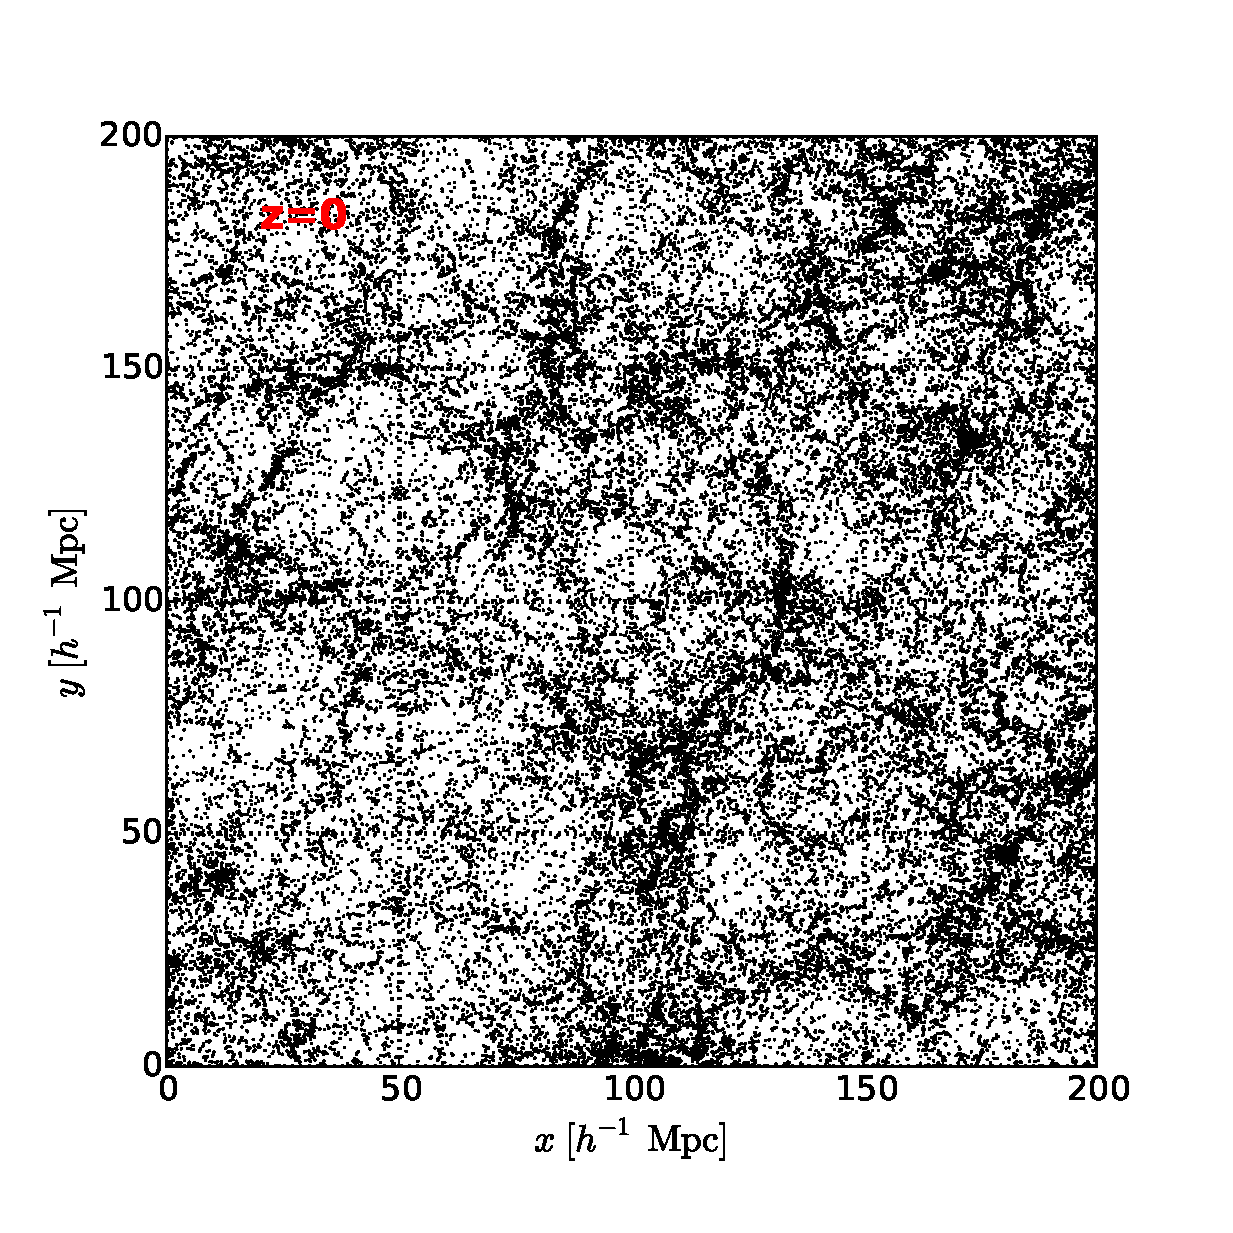
\includegraphics[height=5.9cm]{fig8_0.eps}
   %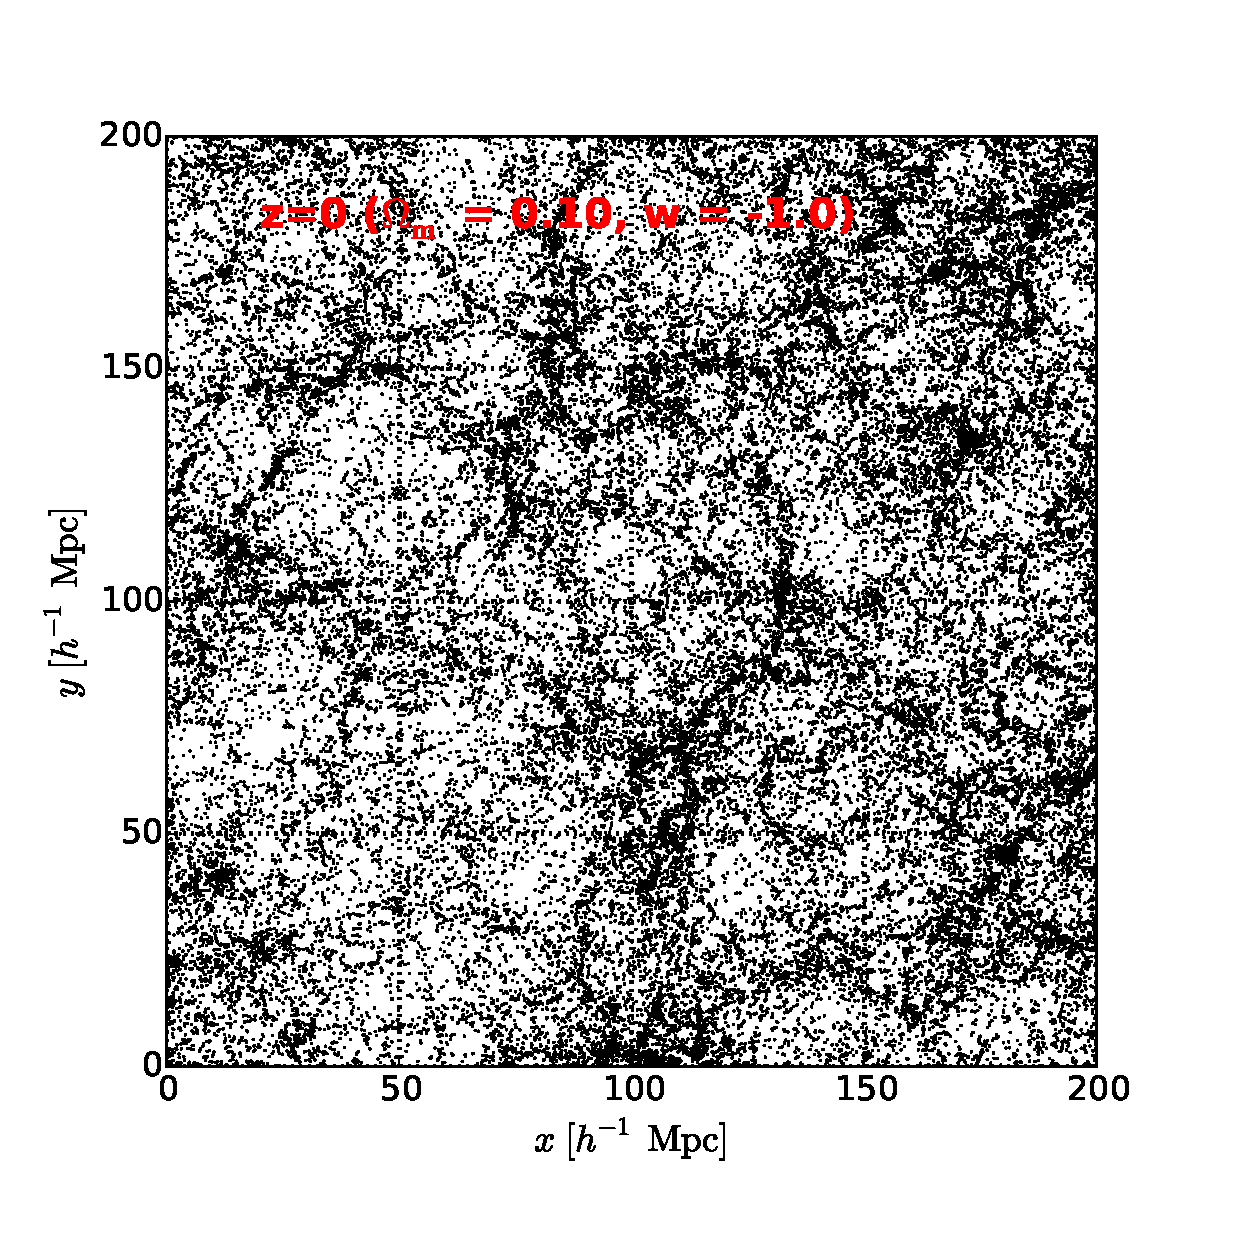
\includegraphics[height=5.9cm]{fig8_wrongcos_0.eps}
   %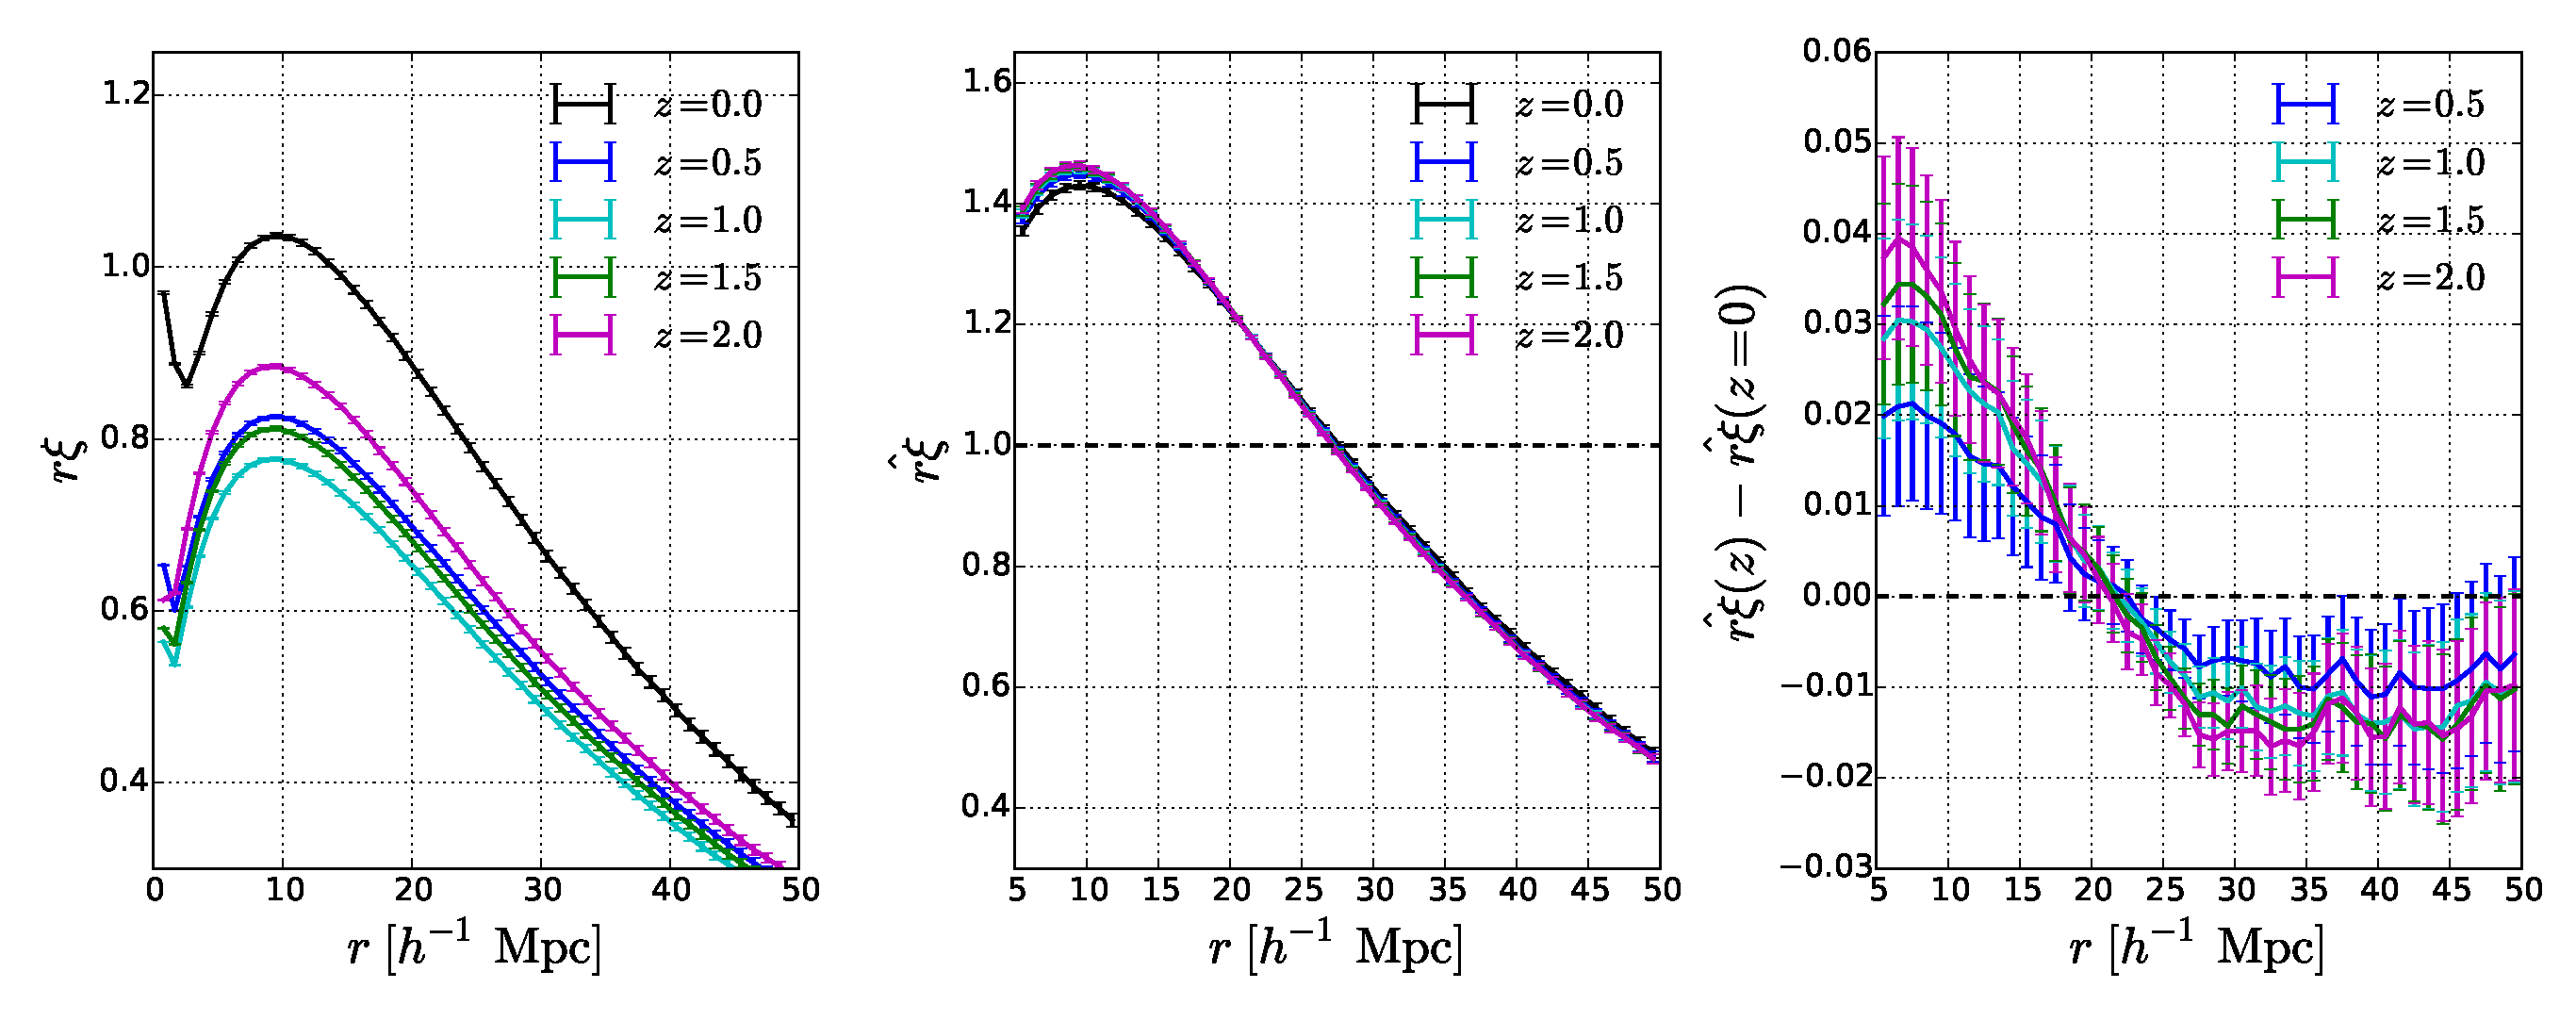
\includegraphics[width=16cm]{fig2.eps}
   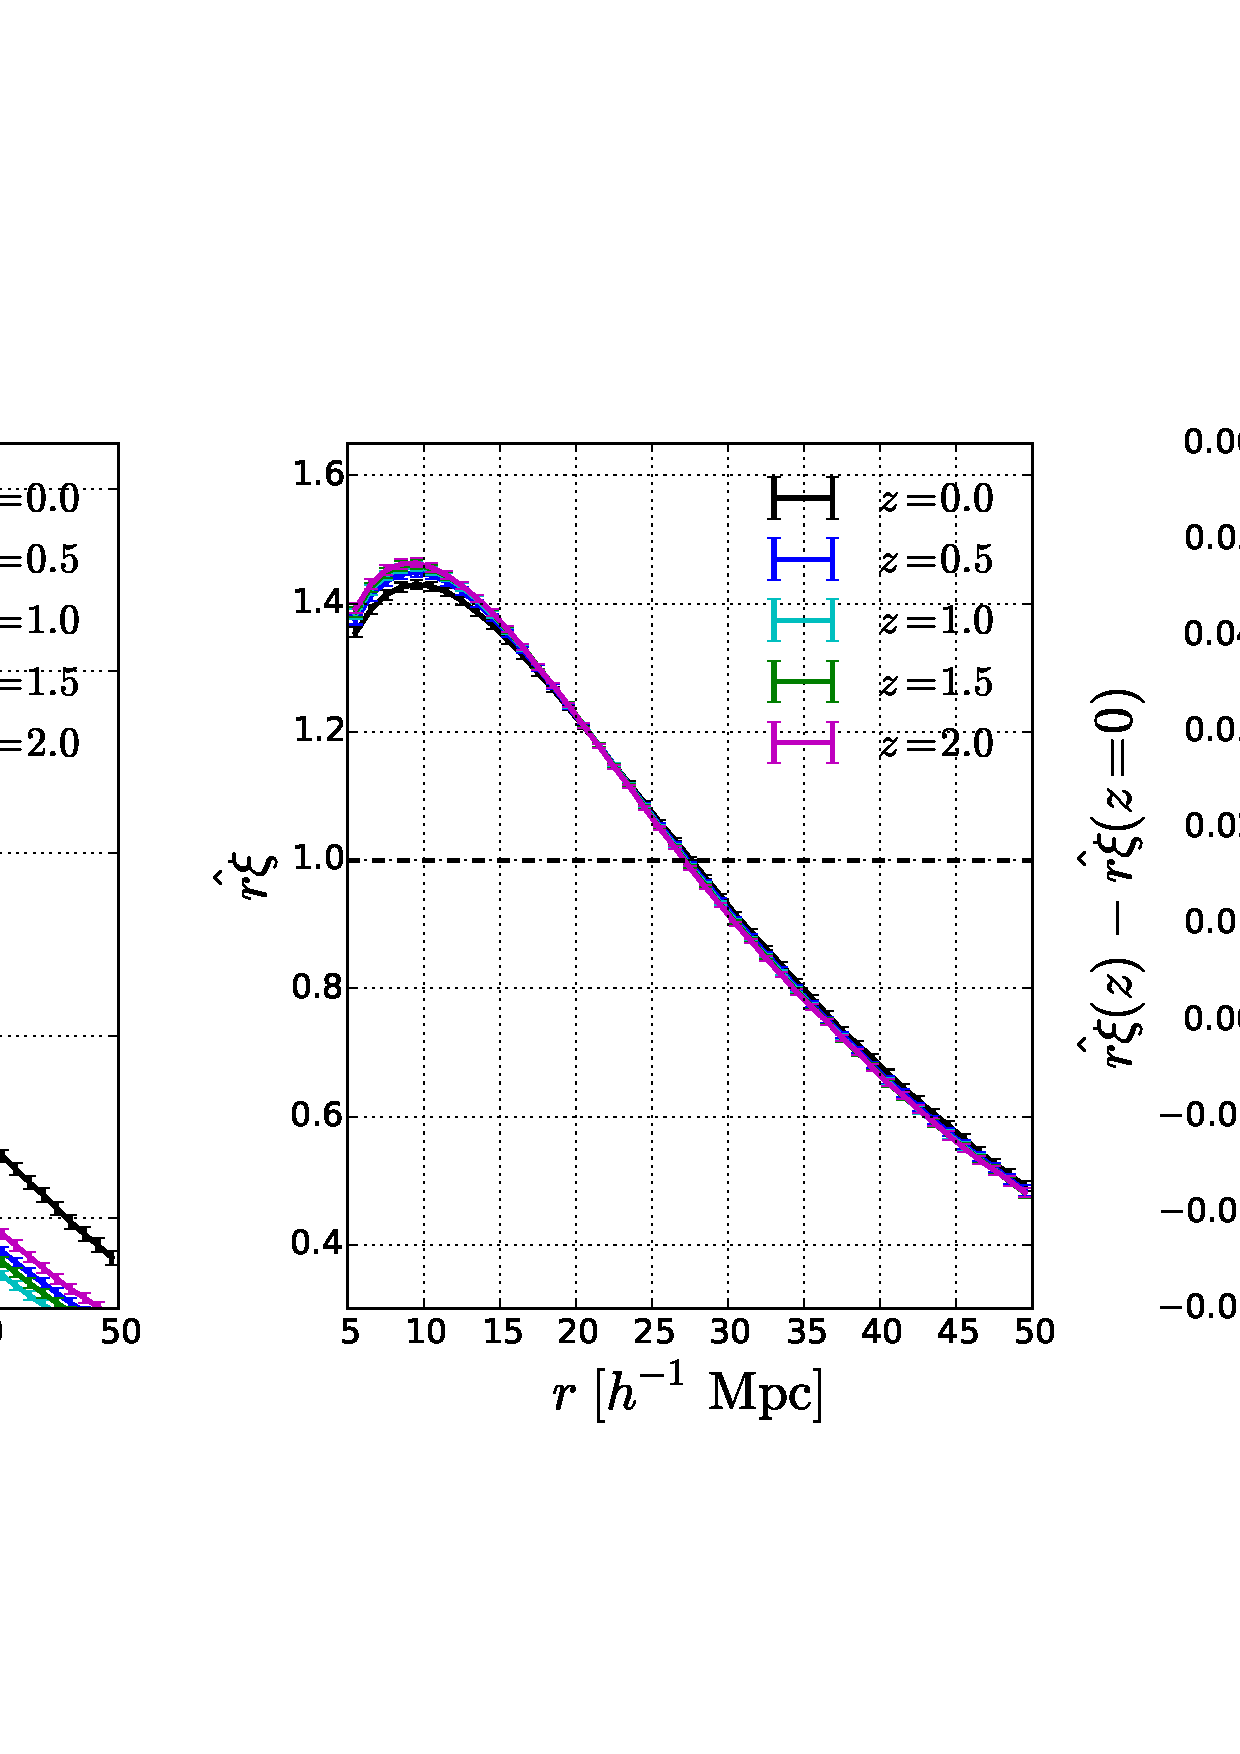
\includegraphics[width=16cm,natwidth=8,natheight=14]{fig2.pdf}
   }
   \caption{\label{fig_scatter}
  blah
   }
   % Need a better plot to show angular size variation!!!
\end{figure*}


\subsection{Galaxy angular 2pCF: amplitude and shape at different redshifts}


\begin{figure*}
   \centering{
%   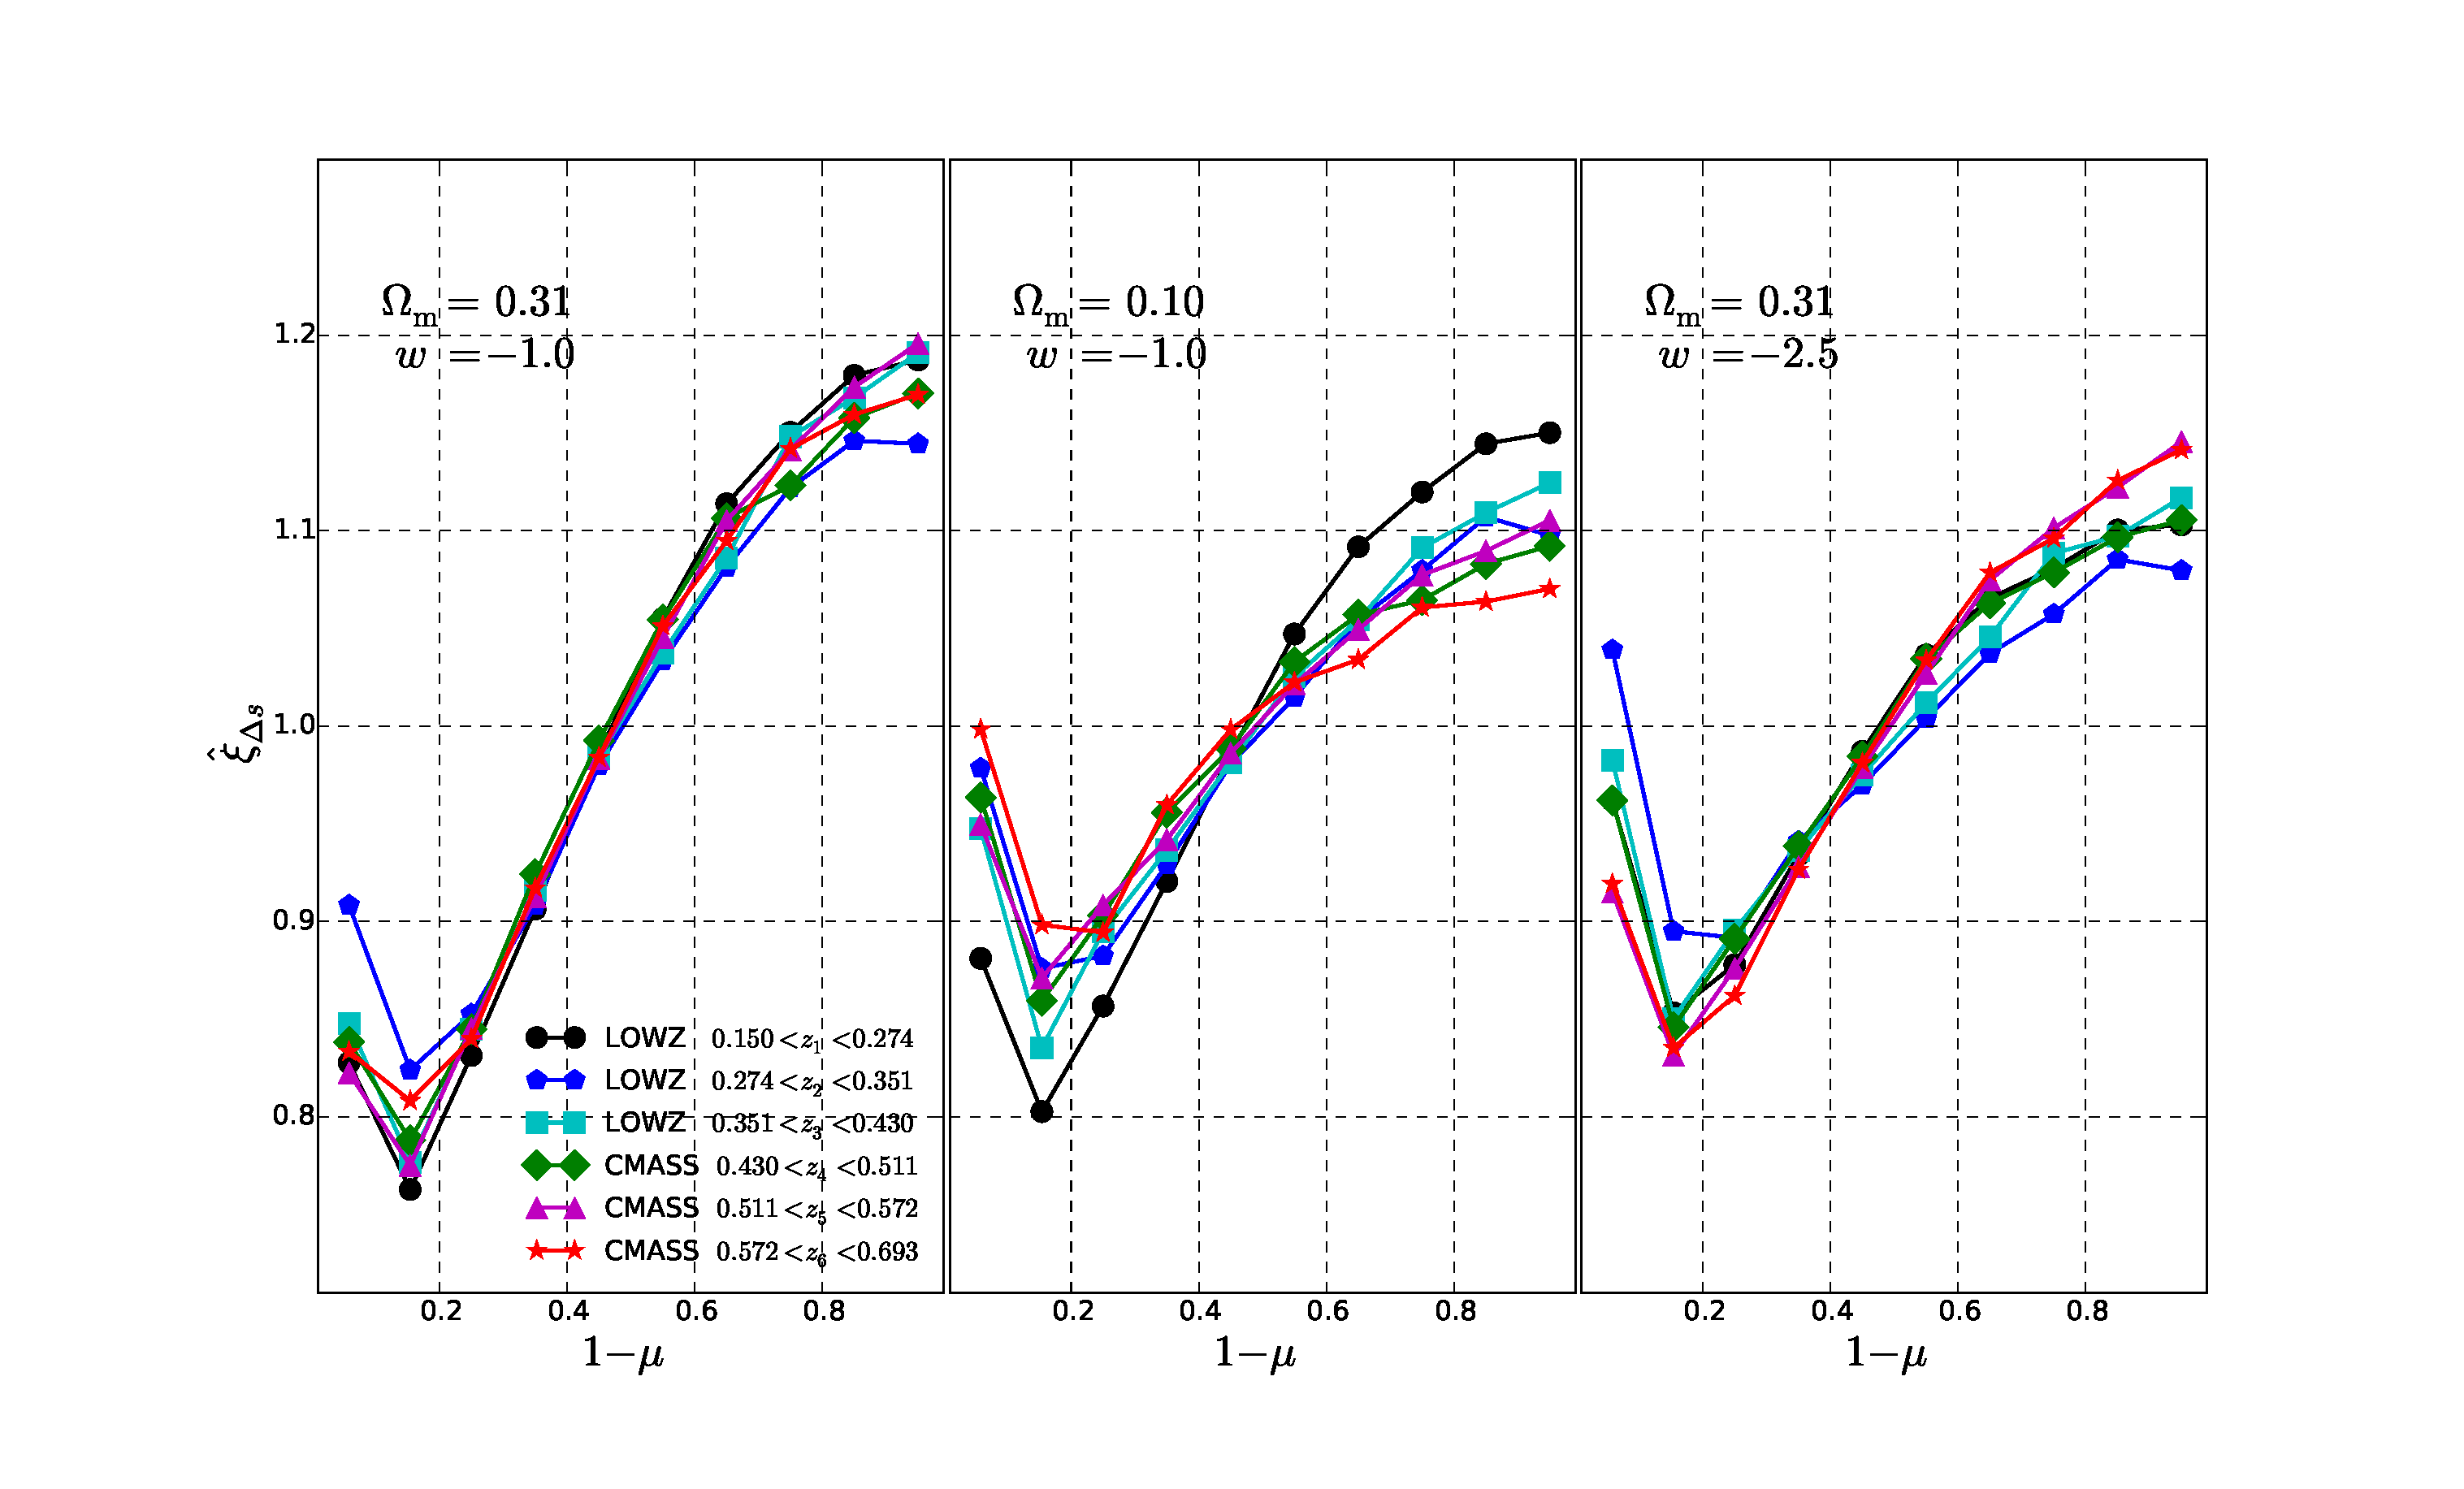
\includegraphics[width=18cm]{fig9_0.eps}
%   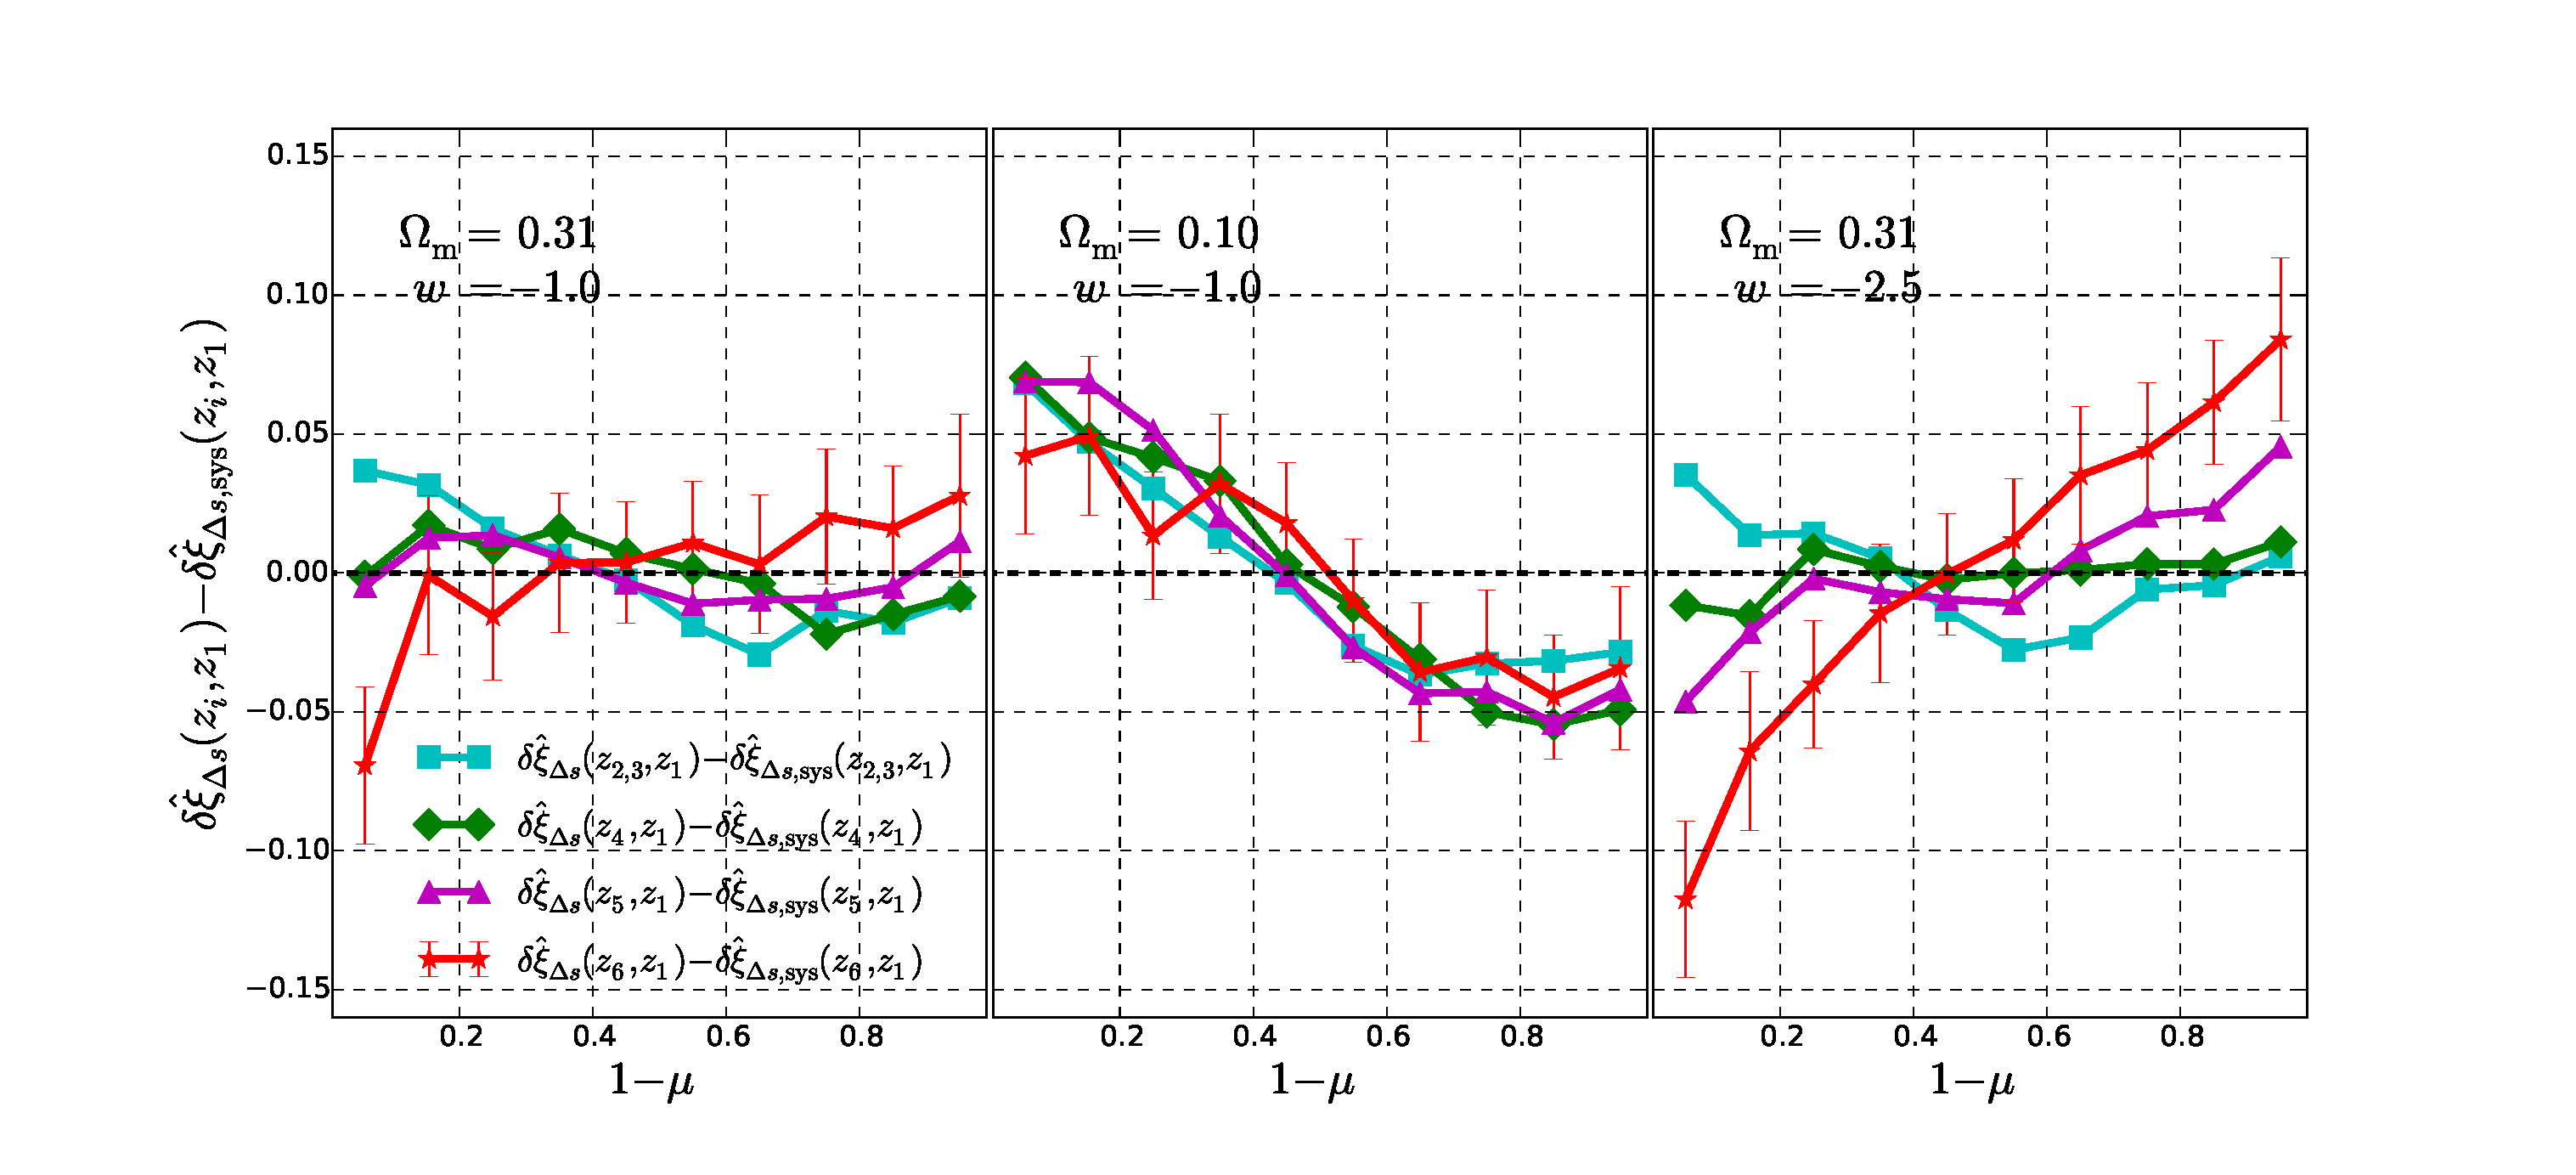
\includegraphics[width=18cm]{fig9_1.eps}
%   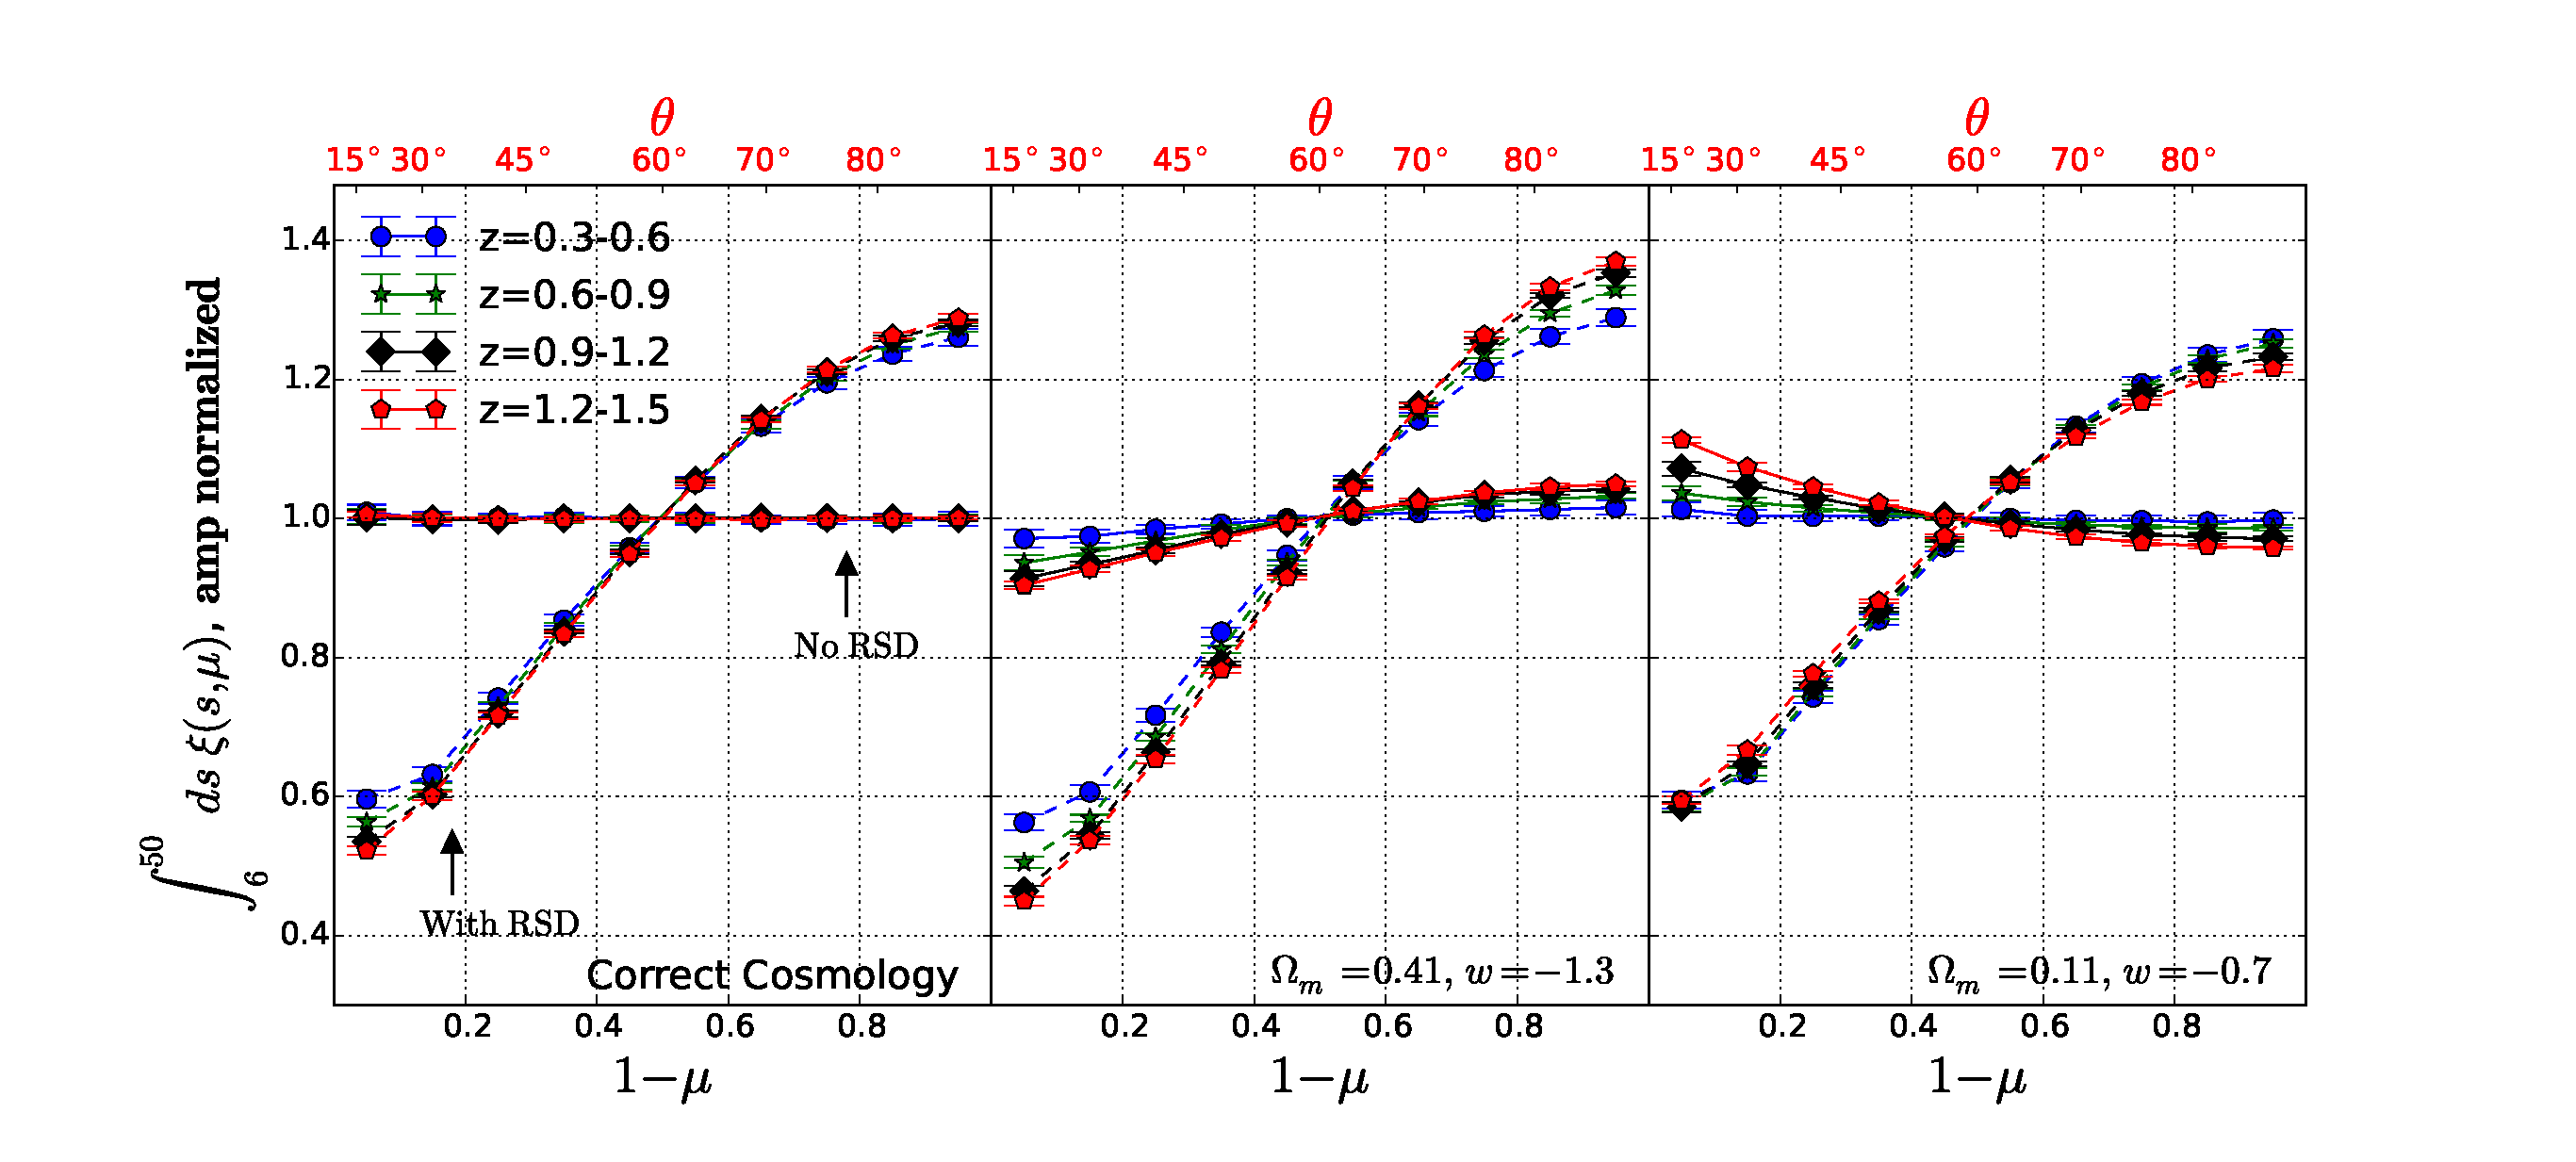
\includegraphics[height=8cm]{Tpcf--plot--Normed.eps}
%    \includegraphics[height=8cm]{smu.eps}
    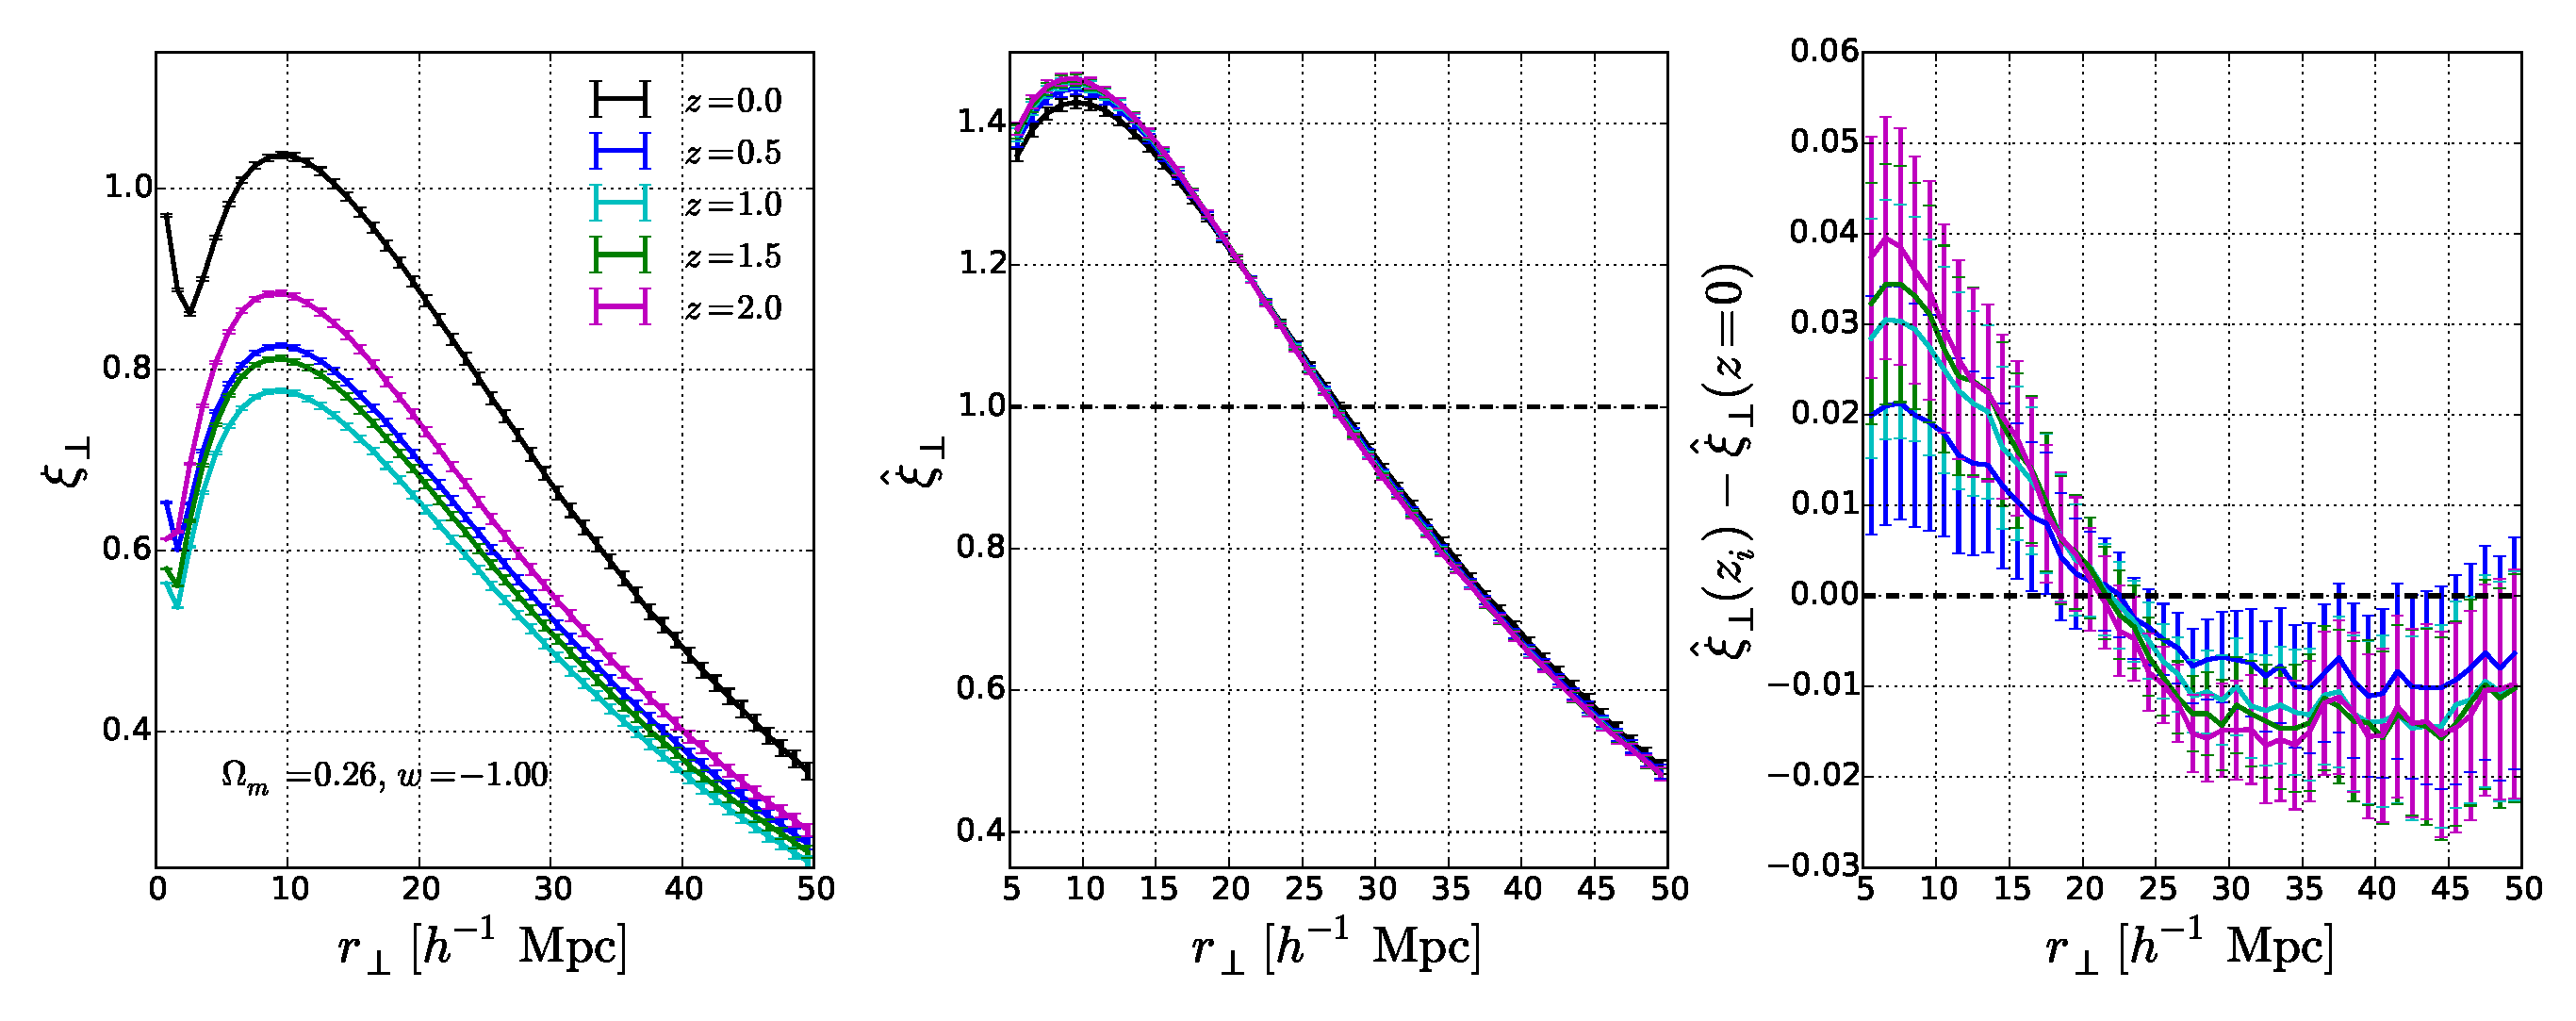
\includegraphics[width=18cm]{fig3.eps}
    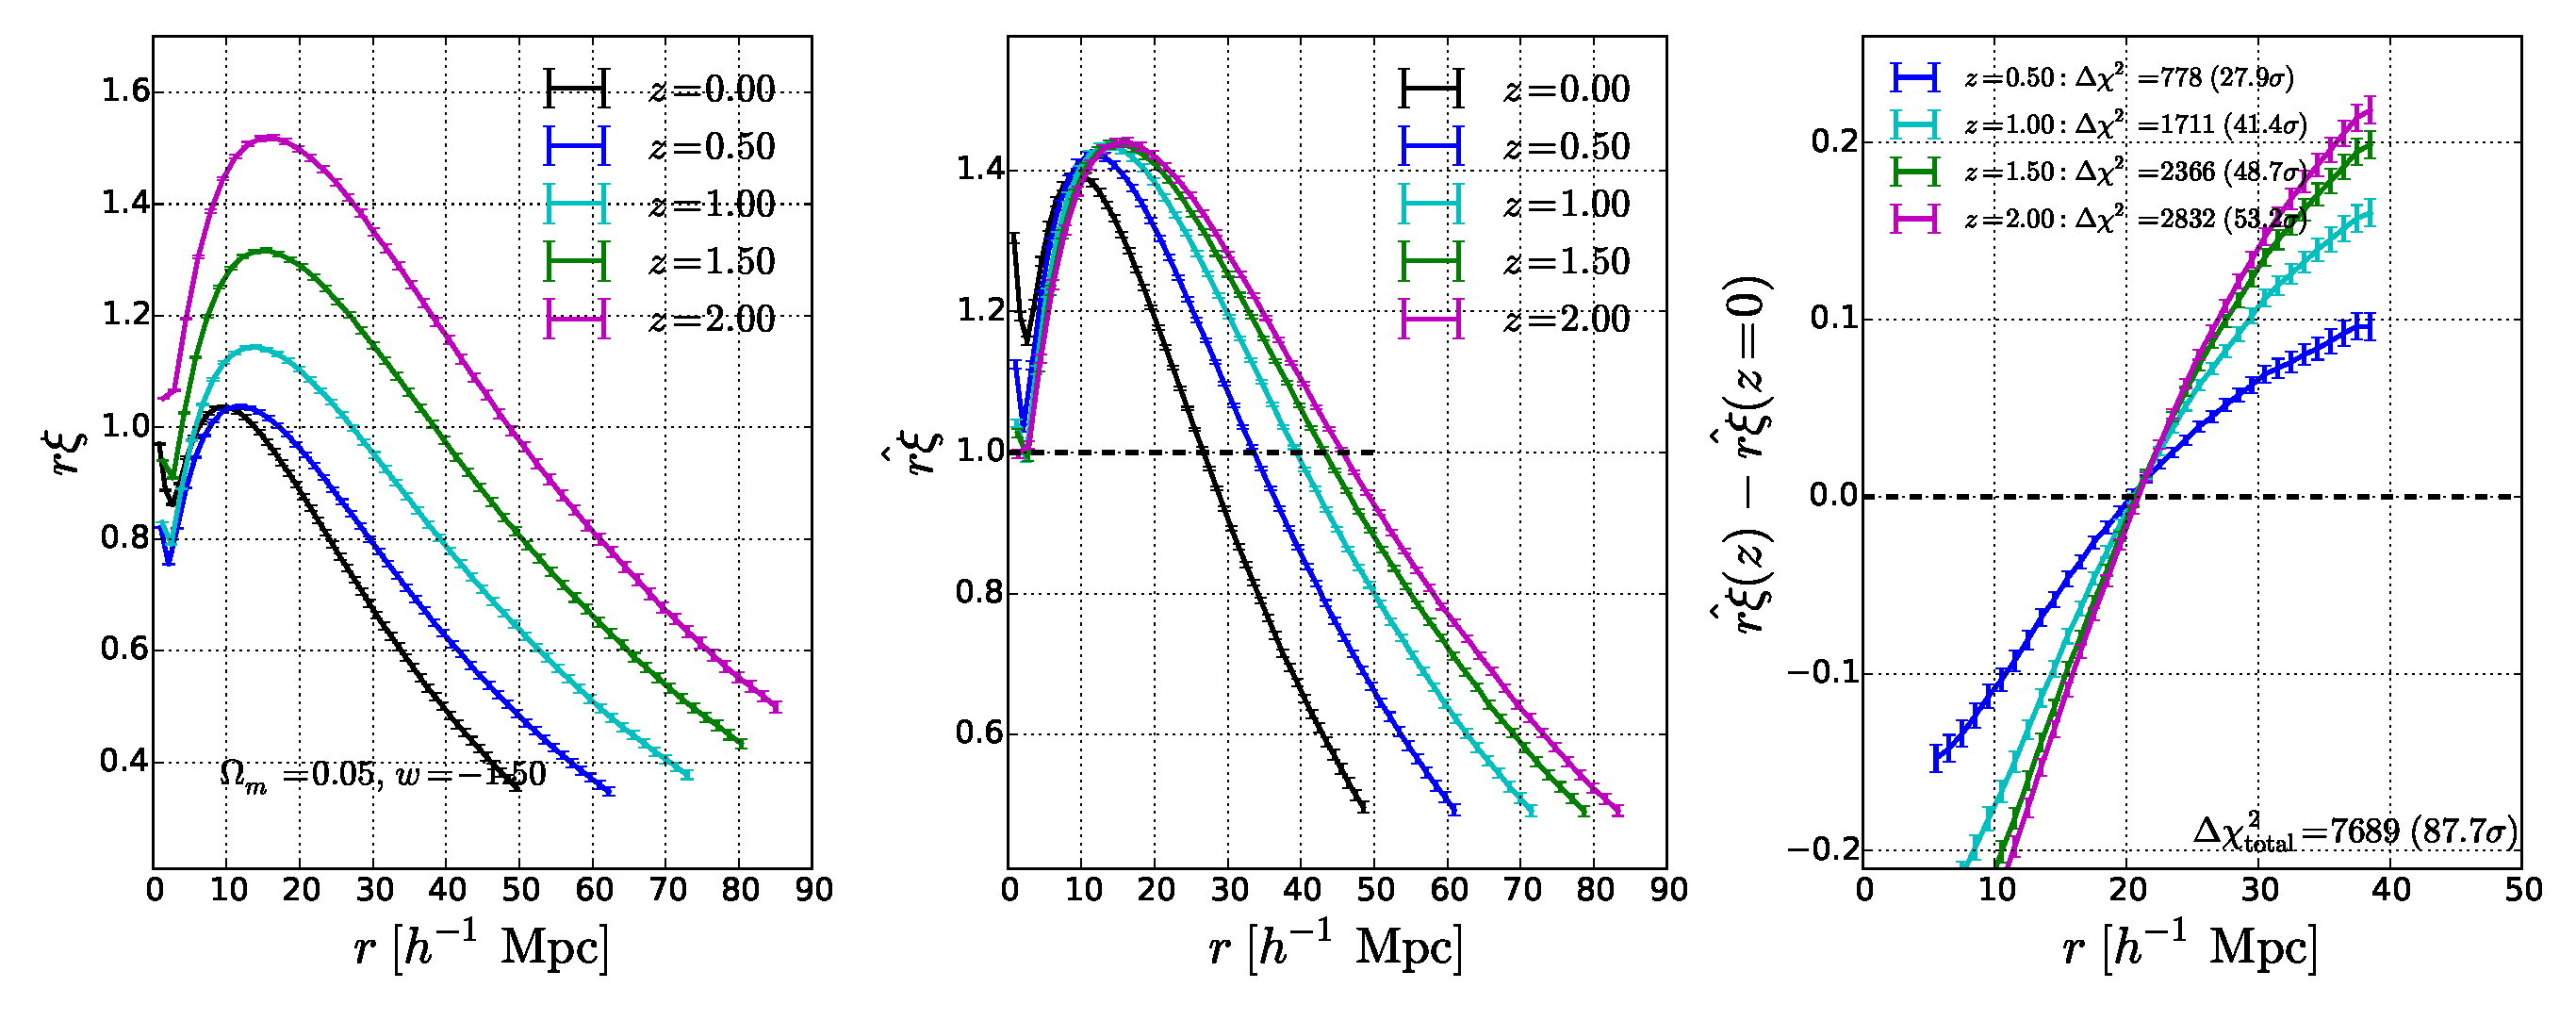
\includegraphics[width=18cm]{fig3_b.eps}
   }
   \caption{\label{fig_diffz}
  2pCF at different redshfits.
   }
\end{figure*}

The left panel of Figure \ref{fig_diffz} displays the measured angular 2pCF of galaxies (multiplied by scale $r$) in the five snapshot.

The amplitude of 2pCF is crucially affected by the cosmic structure growth and the galaxy bias.
%The amplitude is higher at $z=0$, 
We find $\xi(z=0)>\xi(z=0.5)>\xi(z=1)$.
At low redshift, the large scale structures experienced most gravitational growth,
leading to stronger clustering strength and higher amplitude of 2pCF.
On the contrary, at higher redshift we find $\xi(z=2)>\xi(z=1.5)>\xi(z=1)$,
%The trend is different from $z=1,1.5,2$,
simply because by applying a uniform mass cut we are selecting more biased galaxies at higher redshift.

Different from the large variation of amplitude among the different redshifts, %The shape of $r\xi$ also evolves with redshift.
the shape of 2pCF maintains similar at all redshifts. 
At all redshifts, we see the $r\xi$ peaks at $r\sim9 h^{-1}\rm Mpc$,
and monotonically drops at larger or smaller scales.
The only exception is the relative enhancement of 2pCF at $r\lesssim 2 h^{-1}\rm Mpc$,
which is caused by the non-linear growth of structures on small scales 
and becomes more dramatic at lower redshfit.

The middle panel of Figure \ref{fig_diffz} displays the $r\xi$ normalized by the overall amplitude within $5h^{-1}{\rm Mpc} < r < 50h^{-1}{\rm Mpc}$
(here after $\hat r\xi$).
The nice overlapping of the results from five redshifts 
suggests small evolution of shape with redshift.
In the right panel, we compare the high redshift $\hat r\xi$ 
to the $z=0$ result.
There is 1-4\% relative enhancement 
at $r<10h^{-1}\rm Mpc$,
and $<1.5\%$ relative suppression at $r>25 h^{-1}\rm Mpc$.
The trend is monotonic with redshift.

In all, we conclude that the shape of the 2pCF is more robust than the amplitude against redshift and galaxy bias.

\subsection{Galaxy angular 2pCF: in wrong cosmologies }

When a wrong set of cosmological parameters is adopted,
the galaxy distribution is artificially scaled.
This scaling is expected to change the shape of the 2pCF,
following the relationship,
\begin{equation}
 \hat \xi_{\rm wrong}(r) = \hat\xi_{\rm true}(\alpha_{\bot} r),
\end{equation}
a simple consequence of the fact that clustering patterns at distance $r$ now appears on a the scale $\alpha_{\bot} r$.
The redshift evolution of $\alpha_{\bot}$ leads to redshfit evolution of shape.


Lower panels of Figure \ref{fig_diffz} shows the $r\xi$ in five 
snapshots, in case that the cosmology $\Omega_m=0.05,\ w=-1.5$ 
is adopted to construct the galaxy distribution (the right panels of Figure \ref{fig_scatter}).
The middle panel displays the clear redshift evolution of shape of $r\xi$.
E.g, from $z=0$ to $z=2$,
the peak location is shifted from $r=9h^{-1} \rm Mpc$ to $r\sim15 h^{-1}\rm Mpc$ at $z=2$
since the angular separation is upscaled by $71.7\%$.

The right panel shows that, 
at higher redshift, 
there is a 20-40\% change in the value of $\hat {r\xi}$.

The amplitude of $r\xi$ is amplified due to the stretch of scale.
As shown in the left panel, the amplitude monotonically increases as a function of redshift.
But this phenomenon can also appear in case of gravitational growth of structure or increasing of bias,
so we will not make use of it to do cosmological constraint.
We utilize the redshift evolution of the 2pCF shape as a signal suggesting that the assumed cosmological parameters are wrong.

In Figure \ref{fig_cosmo} we further plot the redshift evolution of 2pCF in the four wrong cosmologies of Figure \ref{fig_xyquan}.
In all cases, the scaling leads to evident redshift evolution of the shape of $r\xi$.
When the cosmologies $\Omega_m=0.4,w=-1$ and $\Omega_m=0.26,w=-0.5$ are adopted,
the compression of structure makes the clustering patterns appears on smaller scales.
This leads to ``steeper'' slope of $r\xi$, 
and the higher the redshift, the steeper the slope.
To the opposite, when adopting the cosmologies $\Omega_m=0.15,w=-1$ and $\Omega_m=0.26,w=-1.5$,
the stretch of size makes the slope shallower at higher redshfits.


\subsection{Systematic effects}

The same as \cite{Li2014,Li2015,Li2016} we need to correct for the redshift evolution of $r\xi$ caused by effects other than the wrongly assumed cosmological parameters.

Figure \ref{fig_diffz} already shows that, the growth of structure, especially in low redshift and on non-linear scales, 
changes the shape of $r\xi$ and caused relative enhancement on $r\lesssim2 h^{-1}\rm Mpc$.
So we limit the region of scale to $r>5h^{-1}\rm Mpc$ to minimize its effect.

Galaxies are biased tracers of dark matter field, 
and more massive galaxies tend to reside in regions with higher density contrast.
So in large scale structure surveys the bias of the galaxy sample is an important fator which has large effect on the clustering properties of the sample.
The upper panels of Figure \ref{fig_sys} displays five set of galaxy samples in a $3175\times3175\times105$ $(h^{-1}\rm Mpc)^3$ volume, taken from the $z=0$ snapshots data.
Different lower mass limits of $3\times 10^{11} M_{\odot}$, $3\times 10^{11} M_{\odot}$, $3\times 10^{11} M_{\odot}$ and $3\times 10^{11} M_{\odot}$
are imposed to create subsamples with different galaxy bias, 
and the measured angular 2pCF are displayed.
The different mass cuts result in large variation in the amplitude of the 2pCF (left panel),
while the shape of the 2pCF remains less affected (middle panel).
Compared with the sample with mass cut $M>3\times 10^{11} M_{\odot}$,
samples with mass limit $3\times 10^{11} M_{\odot}$, $3\times 10^{11} M_{\odot}$ and $3\times 10^{11} M_{\odot}$
have the amplitude of 2pCFs enhanced by $10\%,\ 50\%$ and $100\%$,
while the change in $\hat{r\xi}$ is only $0.5\%,\ 2\%$ and $4\%$.
Considering the very large change in the mass cut,
the change in the shape of 2pCF is not significant.

The galaxy peculiar velocity contribute to the observed galaxy redshift and distorted the galaxy radial position in redshift space,
known as the redshift space distortion (RSD).
It is the major source of systematics for our analysis of \cite{Li2014,Li2015,Li2016}, where the 3D galaxy distribution is utilized to derive cosmological constraint.
In this analysis its effect becomes much milder since the angular positions of the galaxies is not affected by RSD at all.
But it still affects our analysis in the procedure of preparing the subsamples of galaxies for 2pCF analysis.
The galaxies observed in a survey are split into shells of subsamples, with different redshift ranges, to get the 2pCF at different redshifts.
RSD disortes the galaxy redshift and as a result some galaxies close the boundaries of shells will be distributed to wrong redshift shells.

The lower panel of Figure \ref{fig_sys} displays the RSD effect on 2pCF.
To mimick the effect of RSD we shift the $Z$ coordinates of galaxies according to the relation 
\begin{equation}\label{eq:zvpeu}
\Delta z = (1+z) \frac{v_{{\rm Z}}}{c},
\end{equation}
where $v_{{\rm Z}}$ is the galaxy peculiar velocity in $Z$ direction.
Then we split the whole box into 30 slices with thickness $105h^{-1}\rm Mpc$, 
and measure the angular 2pCF.
The left panel shows that the amplitude of measured 2pCF is enhanced by $\sim 10\%$ in case of considering the RSD effect on spliting samples.
The middle panel shows that the shape of 2pCF is also altered -- the slop is suppressed.
If looking at the redshift evolution,
the curves $\hat{r\xi} - \hat{r\xi}(z=0)$ displayed in the right panel,
they changed a lot compared with the case of no RSD effect (the right panel of Figure \ref{fig_diffz}),
but do not become much larger. %But RSD effect does not introduce large redshfit evolution, although the shape of  is 


Similar to RSD, the redshift errors in survey can affect the subsamples of galaxies by buring the boundaries of shells.
This effect should be properly quantified, especially in case of a photometric survey where the redshift uncertainty can be $\Delta z \\approx 0.02$.

In \cite{Li2014,Li2015,Li2016}, the systematic effects contributing to the redshfit evolution of galaxy clusterings 
are modeled in mock surveys and subtracted.
Similar treatment could be conducted here.
One shall construct mock surveys with the above effects included for the correction of systematics.

%The outer boundary of the mock survey becomes fuzzy due to the peculiar velocity effect 
%on the galaxy redshifts (Eq. (\ref{eq:zvpeu})).
%A population of galaxies, that are expected to enter the $z<0.7$ region from the outside, is missing.
%(these $z>0.7$ galaxies have a peculiar velocity toward us and 
%their observed redshfits become lower than 0.7).
%To avoid this problem we set the maximal redshift at 0.693, 
%23.3 $h^{-1}{\rm Mpc}$ away from $z=0.7$.


%3.000e11', '1.000e12', '4.000e12',  '1.000e13



\begin{figure*}
   \centering{
   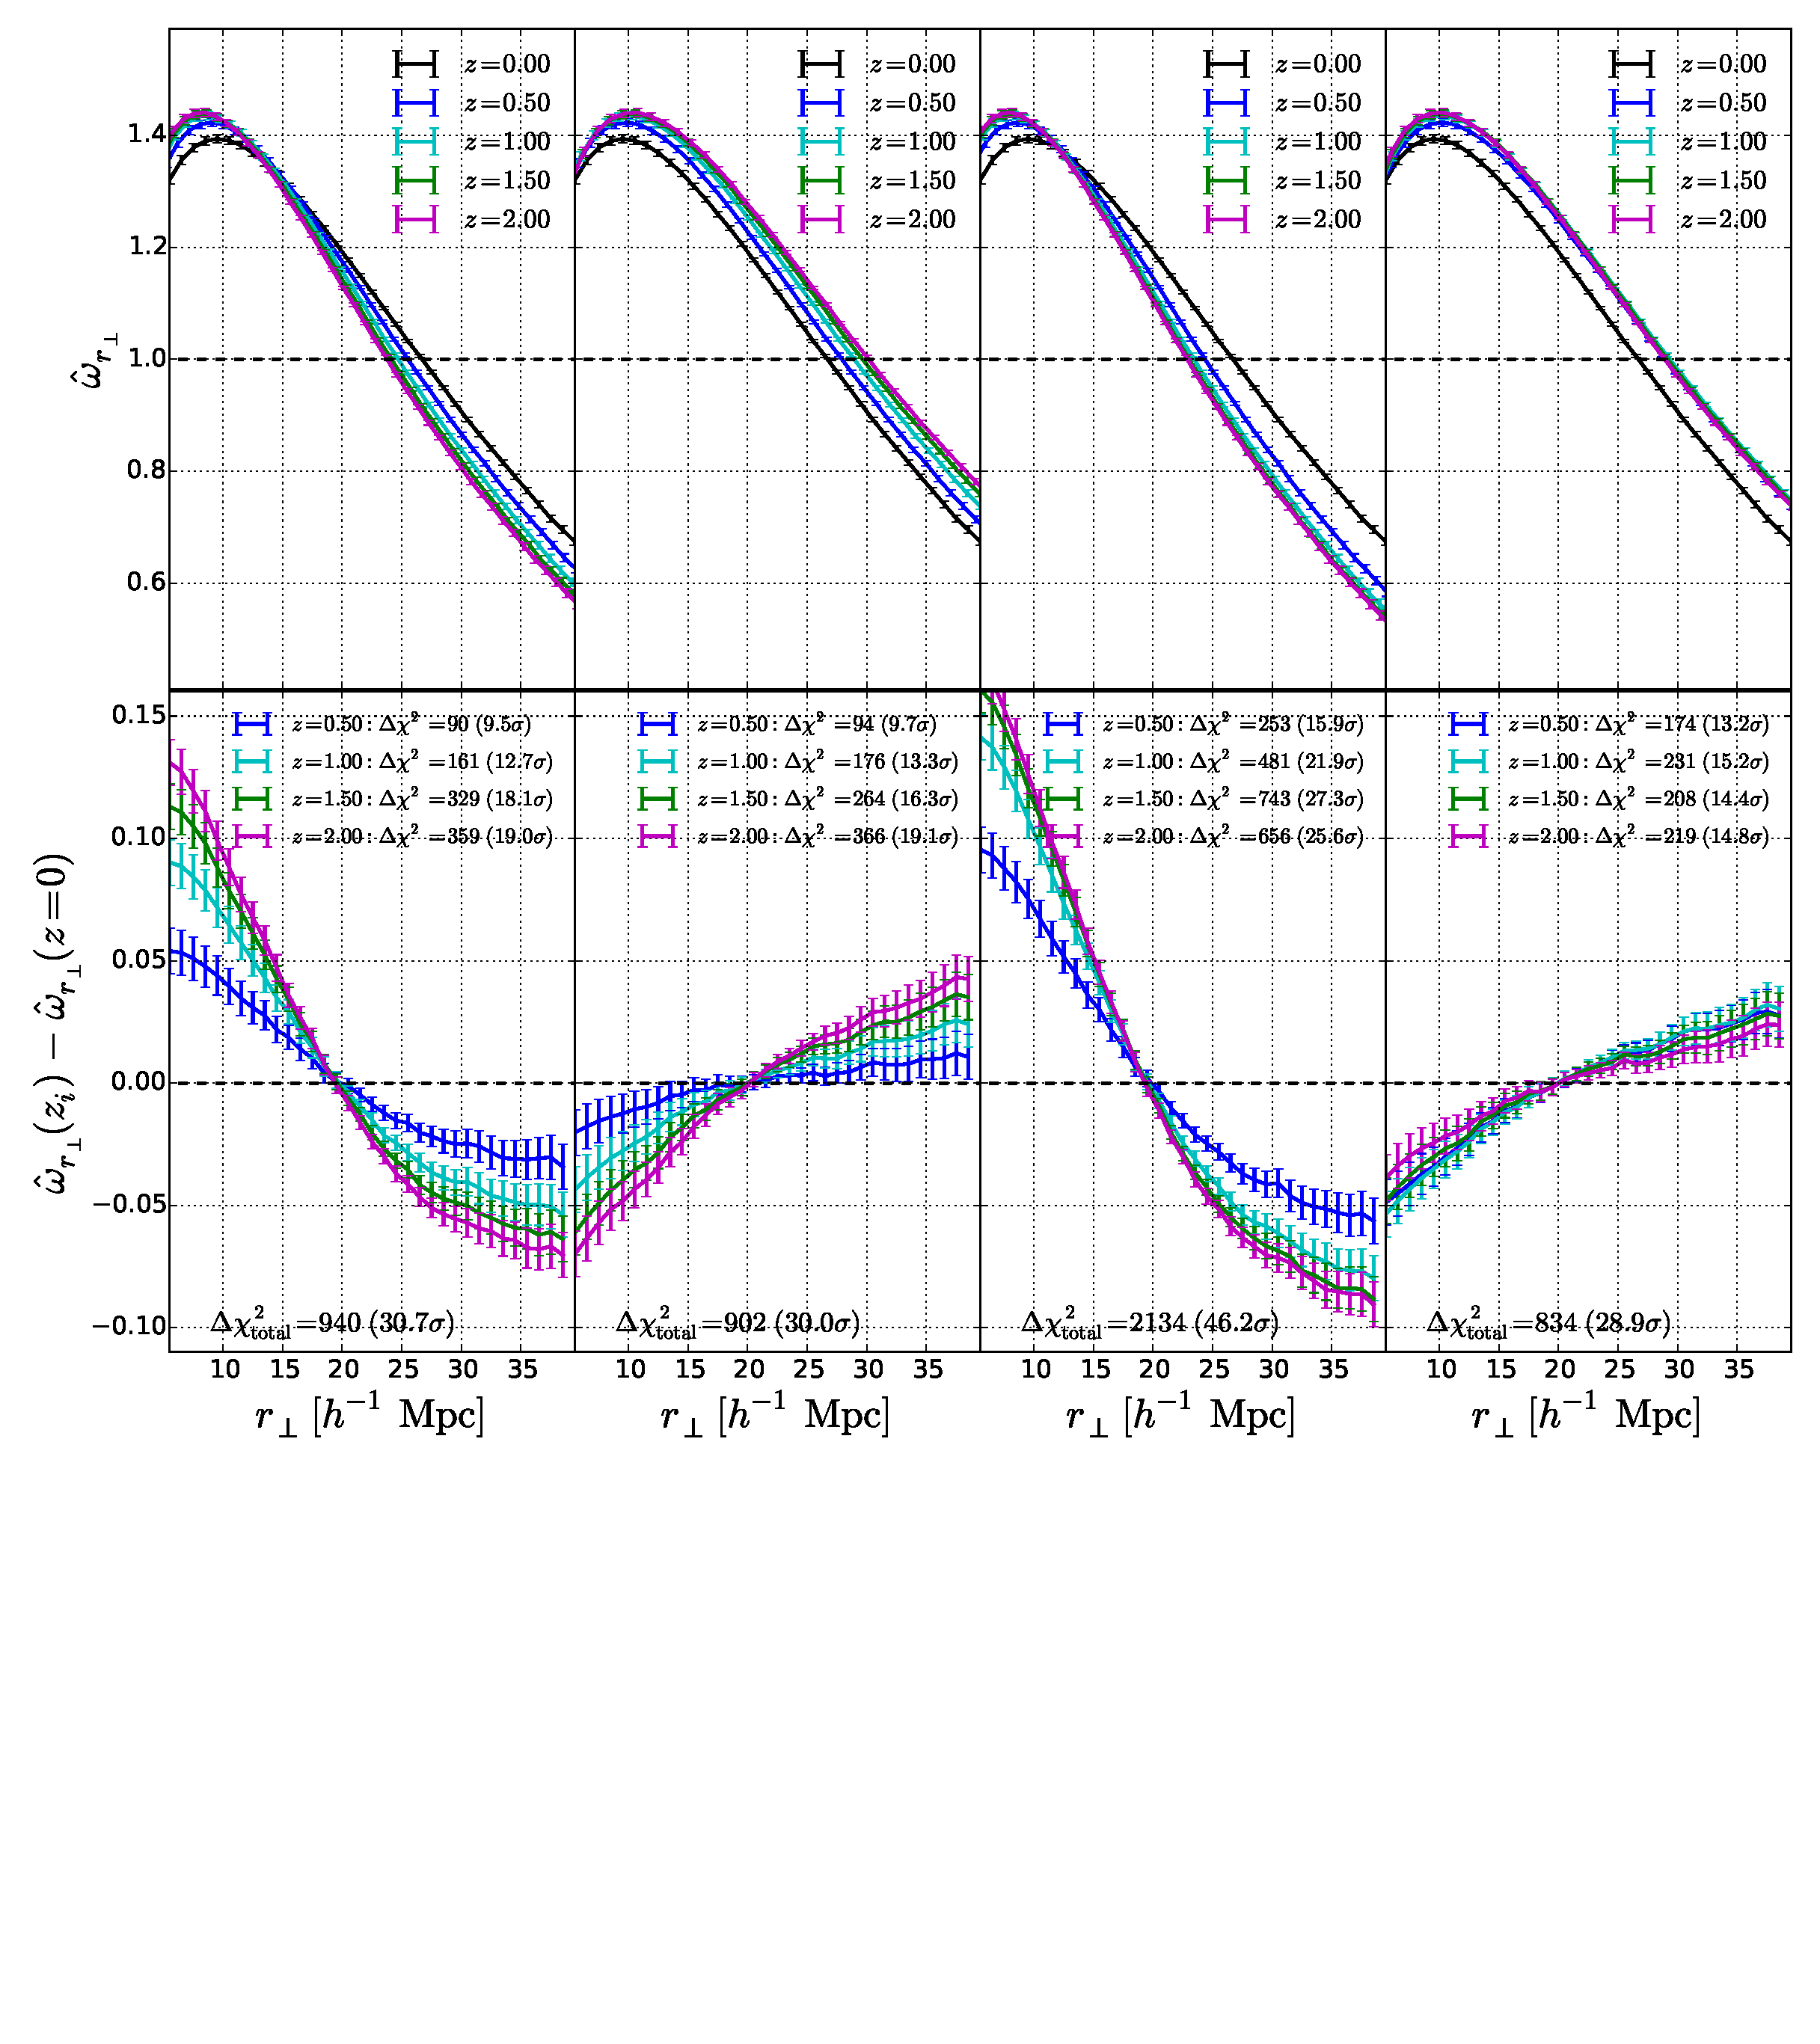
\includegraphics[width=16cm]{fig5.eps}
   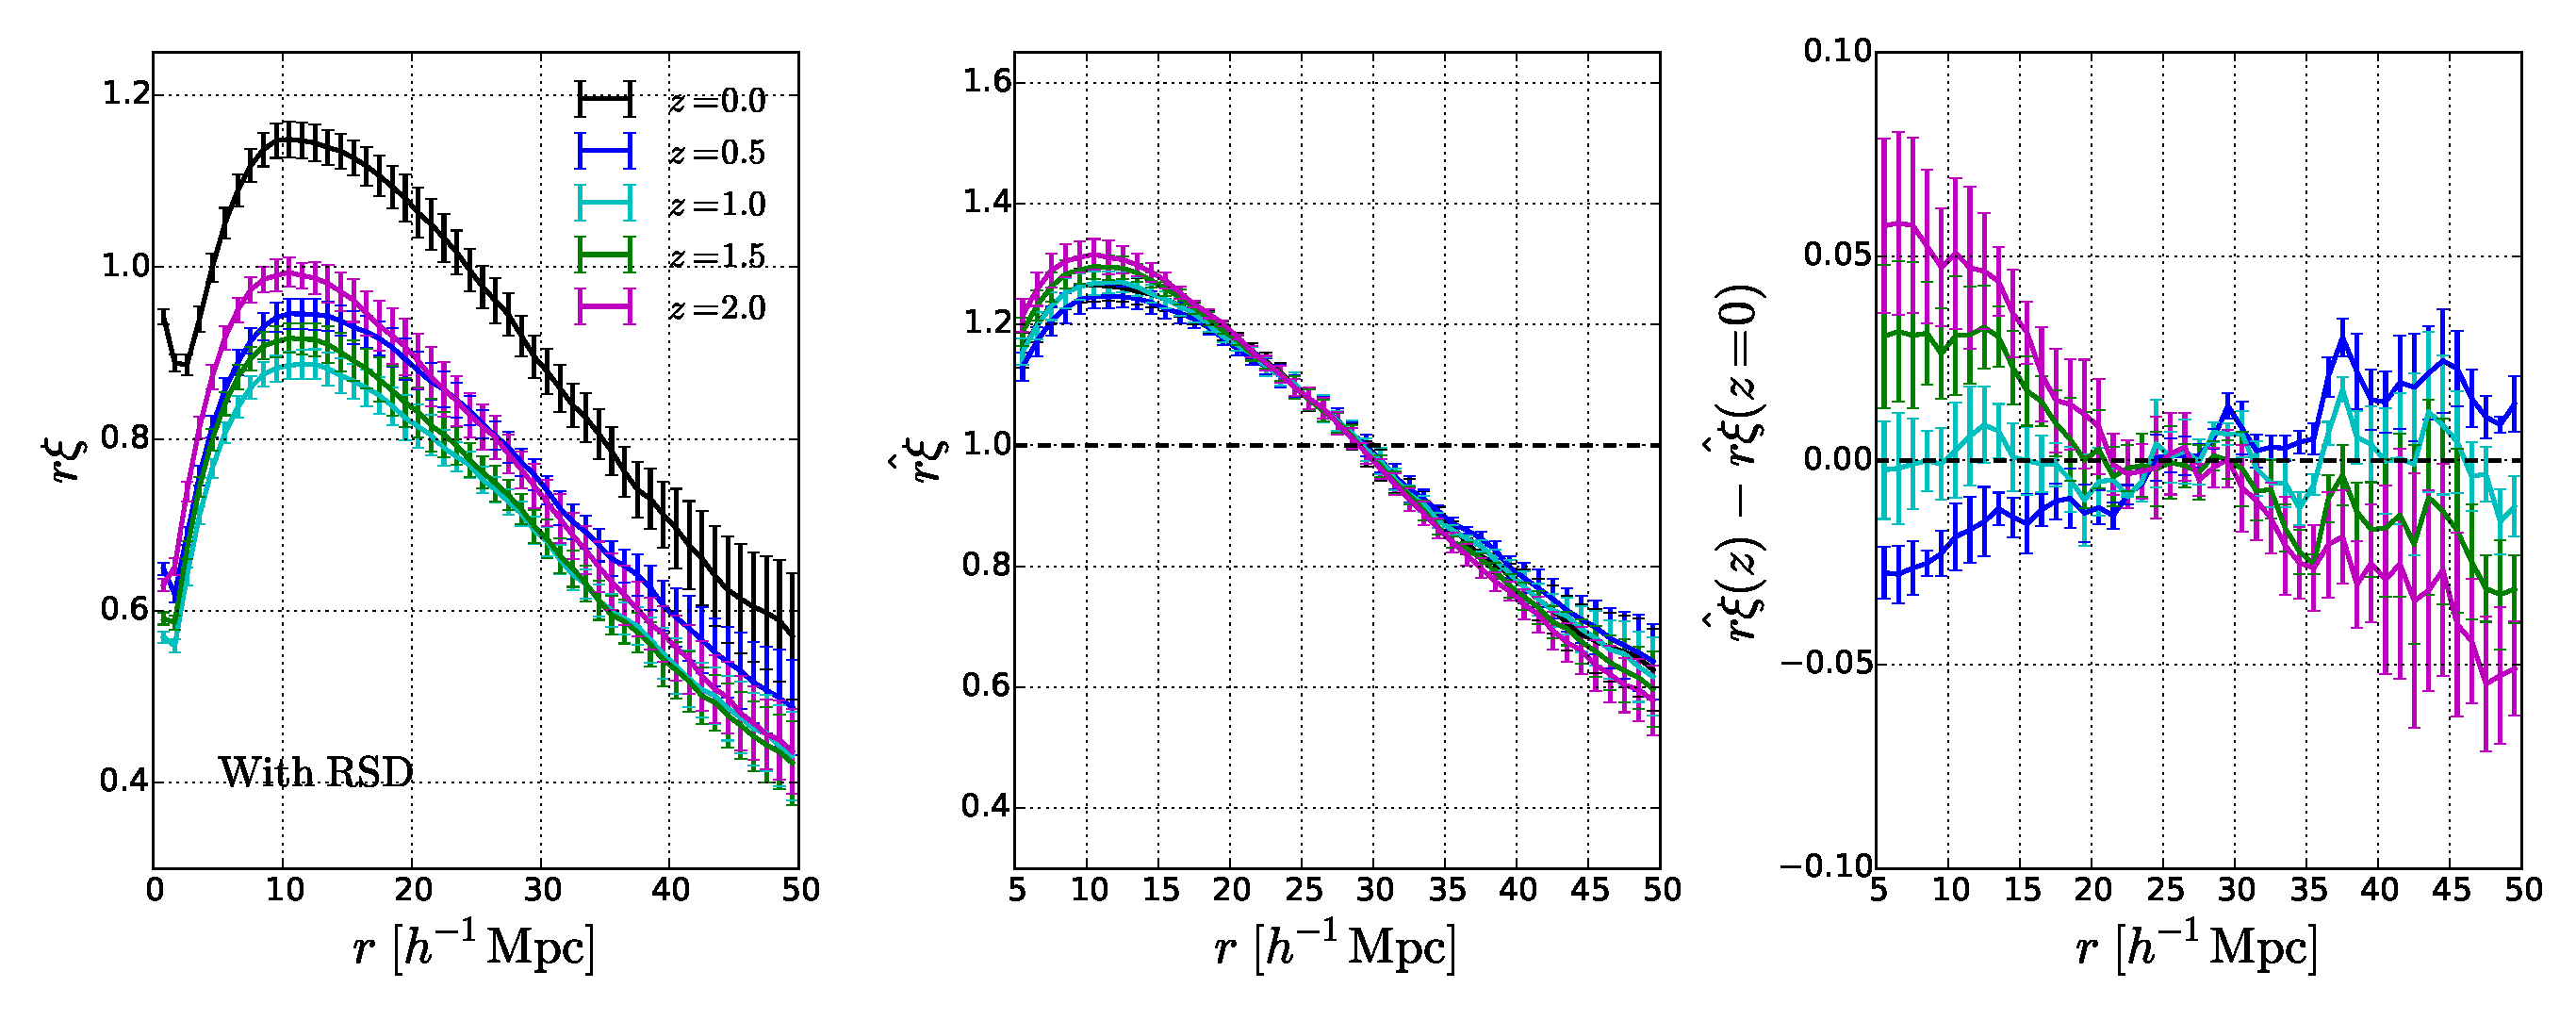
\includegraphics[width=16cm]{fig6.eps}
   }
   \caption{\label{fig_sys}
  Systematic effects.
   }
\end{figure*}


\subsection{Likelihood Analysis}

We build up a likelihood function to 
describe how significant is the redshift evolution of the 2pCF shape,
so that to determine whether the adopted cosmological parameters are correct.
The redshift evolution is characterized by the difference between the $\hat{r\xi}$ measured in the lowest redshift and higher ones;
the cosmology having least redshift evolution of $\hat{r\xi}$ is considered to be the most plausible one and has smallest $\chi^2$.
So we have
\begin{equation}\label{eq:chisq1}
\chi^2\equiv \sum_{i=2}^{n_{z}} \sum_{j_1=1}^{n_{r}} \sum_{j_2=1}^{n_{r}} {\bf p}(z_i,r_{j_1}) ({\bf Cov}_{i}^{-1})_{j_1,j_2}  {\bf p}(z_i,r_{j_2}),
\end{equation}
where $n_z$ is the number of redshifts, 
is number of bins in $\hat{r\xi(r)}$;
in this analysis we have five redshift bins, 
and 35 $r$ bins with bin width $1h^{-1}\rm Mpc$ in the range $5h^{-1}{\rm Mpc}<r<40h^{-1}{\rm Mpc}$.
${\bf p}(z_i,r_{j})$ is the redshift evolution of clustering, 
$\hat {r\xi}$, with systematic effects subtracted
\begin{eqnarray}\label{eq:bfp}
 {\bf p}(z_i,r_{j}) \equiv&\ \delta \hat{r\xi}(z_i,z_1,r_j) - \delta \hat{r\xi}_{\rm sys}(z_i,z_1,r_j)
\end{eqnarray}
${\bf Cov}_i$ is the covariance matrix.

It is difficult to conduct the 2pCF of the whole snapshot box with hundreds of millions of galaxies.
We split the box into 120 subsamples with $X,Y,Z$ sizes of $1575h^{-1}{\rm Mpc},1575h^{-1}{\rm Mpc}, 105h^{-1}{\rm Mpc}$
and measure the angular 2pCF in the $X-Y$ plan in these subsamples. 
The average of the 2pCFs are taken as the 2pCF of the whole box.
The covariance matrix is also estimated from these 2pCFs.

In real observations we observe {\it different} objects at different redshfit shells.
To mimick this when calculating the redshift evolution of 2pCF we use subsamples at different positions at different redshfits.
E.g., if for the $z=0$ snapshot we use the $\hat{r\xi}$ measured in the subsample $0h^{-1}{\rm Mpc}<Z<105 h^{-1}{\rm Mpc}$,
at higher redshifts we adopt the $\hat{r\xi}$ measured in a subsample $105h^{-1}{\rm Mpc}<Z<210 h^{-1}{\rm Mpc}$,
and take the difference between them to get $\delta \hat{r\xi}$.
So we are always comparing 2pCF measured from different samples of galaxies.
If simply comparing the 2pCF of a same sample of galaxies at different redshifts, 
one would significantly underestimate the statistical undertainty of $\delta \hat{r\xi}$ by ignoring the cosmic variance
\footnote{The error bars displayed in all figures are estimated from the 120 subsamples and for the error bar of redshift evolution of 2pCF 
we always take the cosmic variance into consideration.}.
%estimated from the 72 sets of PSB mock galaxies identified from HR3 N-body simulation.



Figure \ref{fig_cosmo} displayed the 2pCF measured in the four cosmologies displayed in Figure \ref{fig_xyquan}.
For the cosmologies $\Omega_m=0.4,w=-1$ and $\Omega_m=0.26,w=-0.5$,
the compression of structure rescale large scale clustering patterns into small scales;
the compression becomes more significant at higher redshift.
In these cosmologies we get 2pCFs with steeper slope and, the higher redshift, the steeper.
For $\Omega_m=0.15,w=-1$ and $\Omega_m=0.26,w=-1.5$,
the stretch of structure leads to shallower slope of $\hat{r\xi}$ and, the higher the redshift, the shallower.
In all cosmologies we find significant detection of redshift evolution of $\hat{r\xi}$ (in the lowest panels, $\delta \hat{r\xi}\neq0$).
We computed the $\chi^2$ values according to Equation \ref{eq:chisq1} and found these sets of cosmological parameters are strongly disfacored 
at $\gtrsim30\sigma$ CL.


\begin{figure*}
   \centering{
%   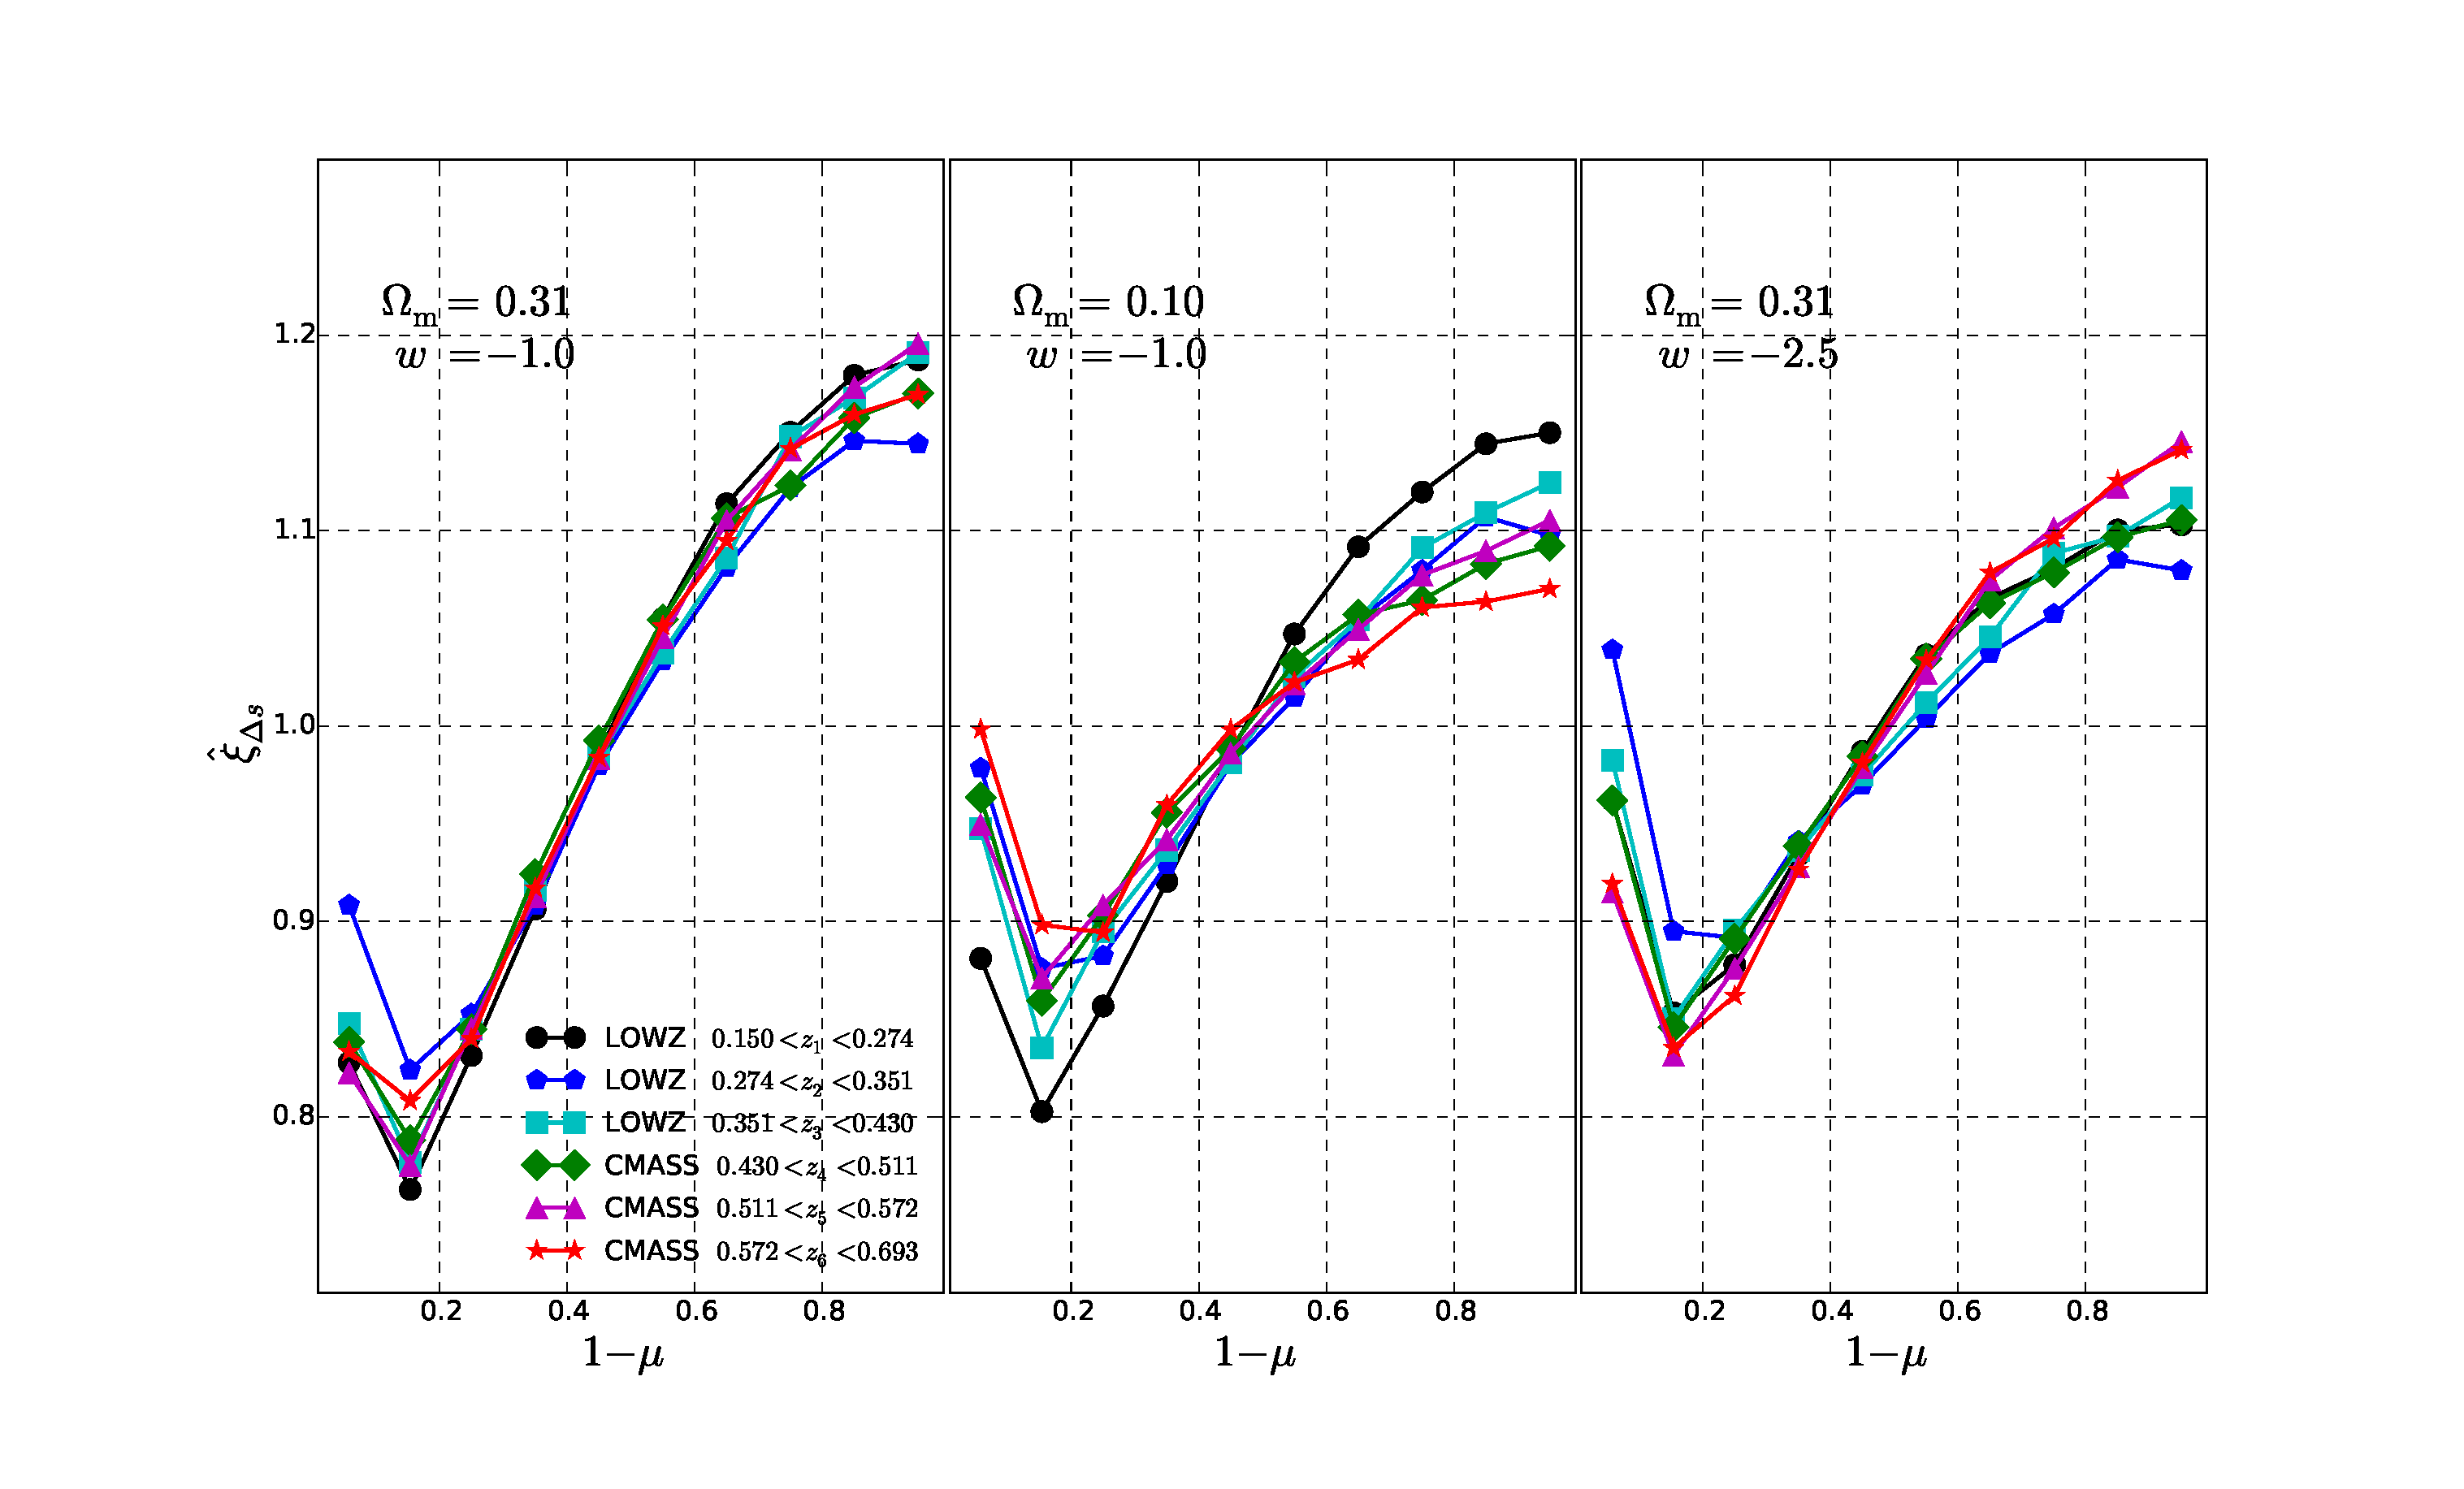
\includegraphics[width=18cm]{fig9_0.eps}
%   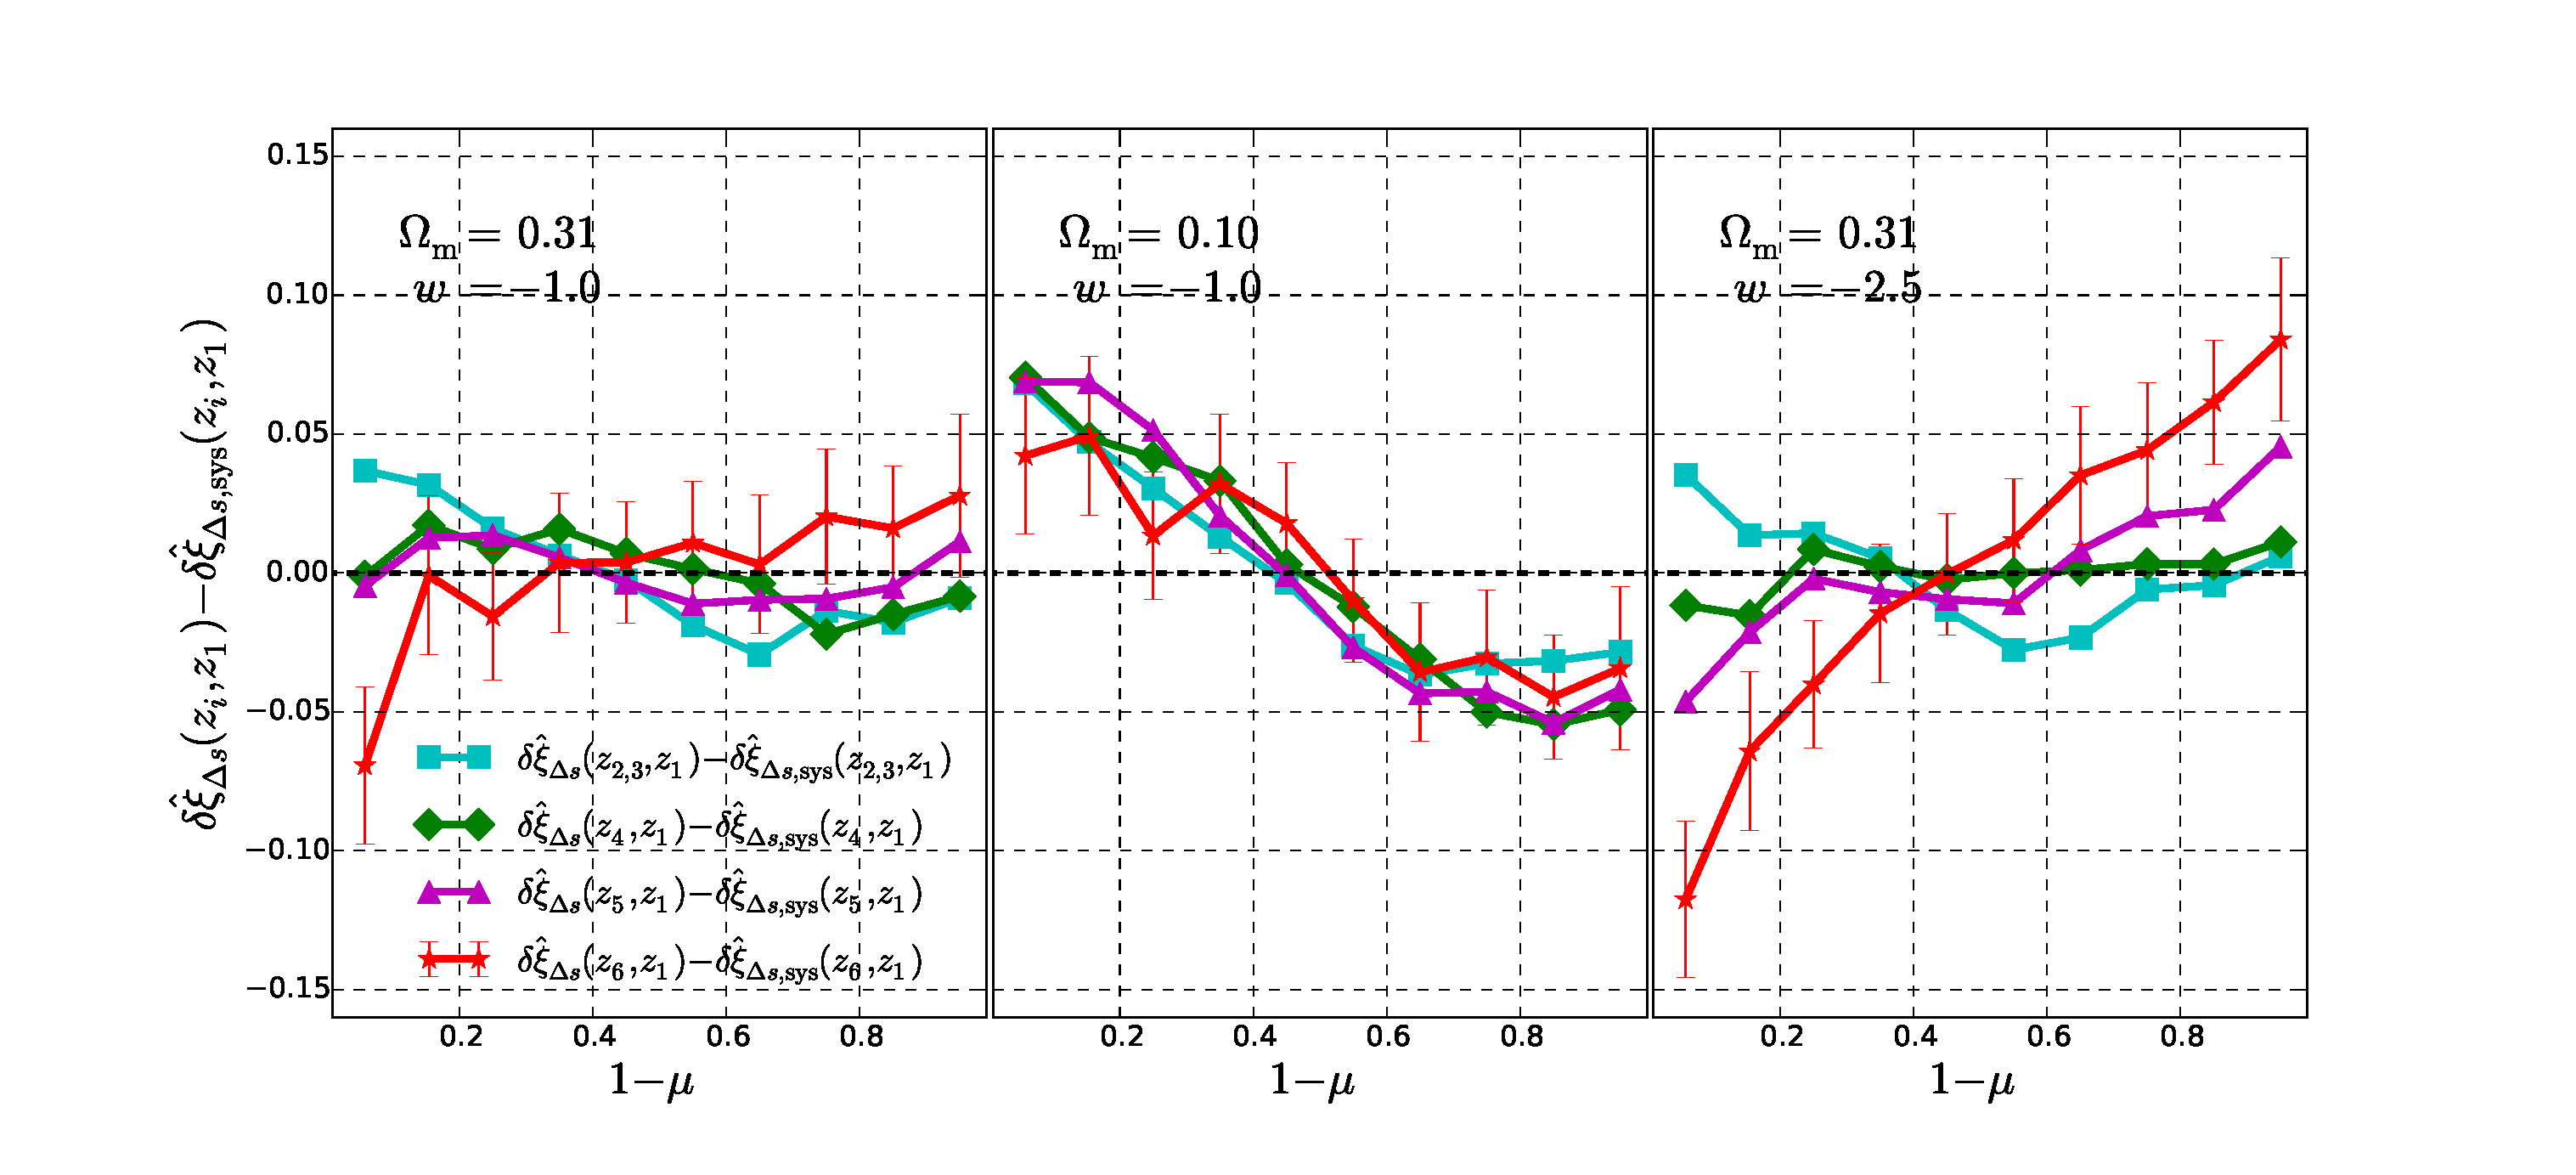
\includegraphics[width=18cm]{fig9_1.eps}
%   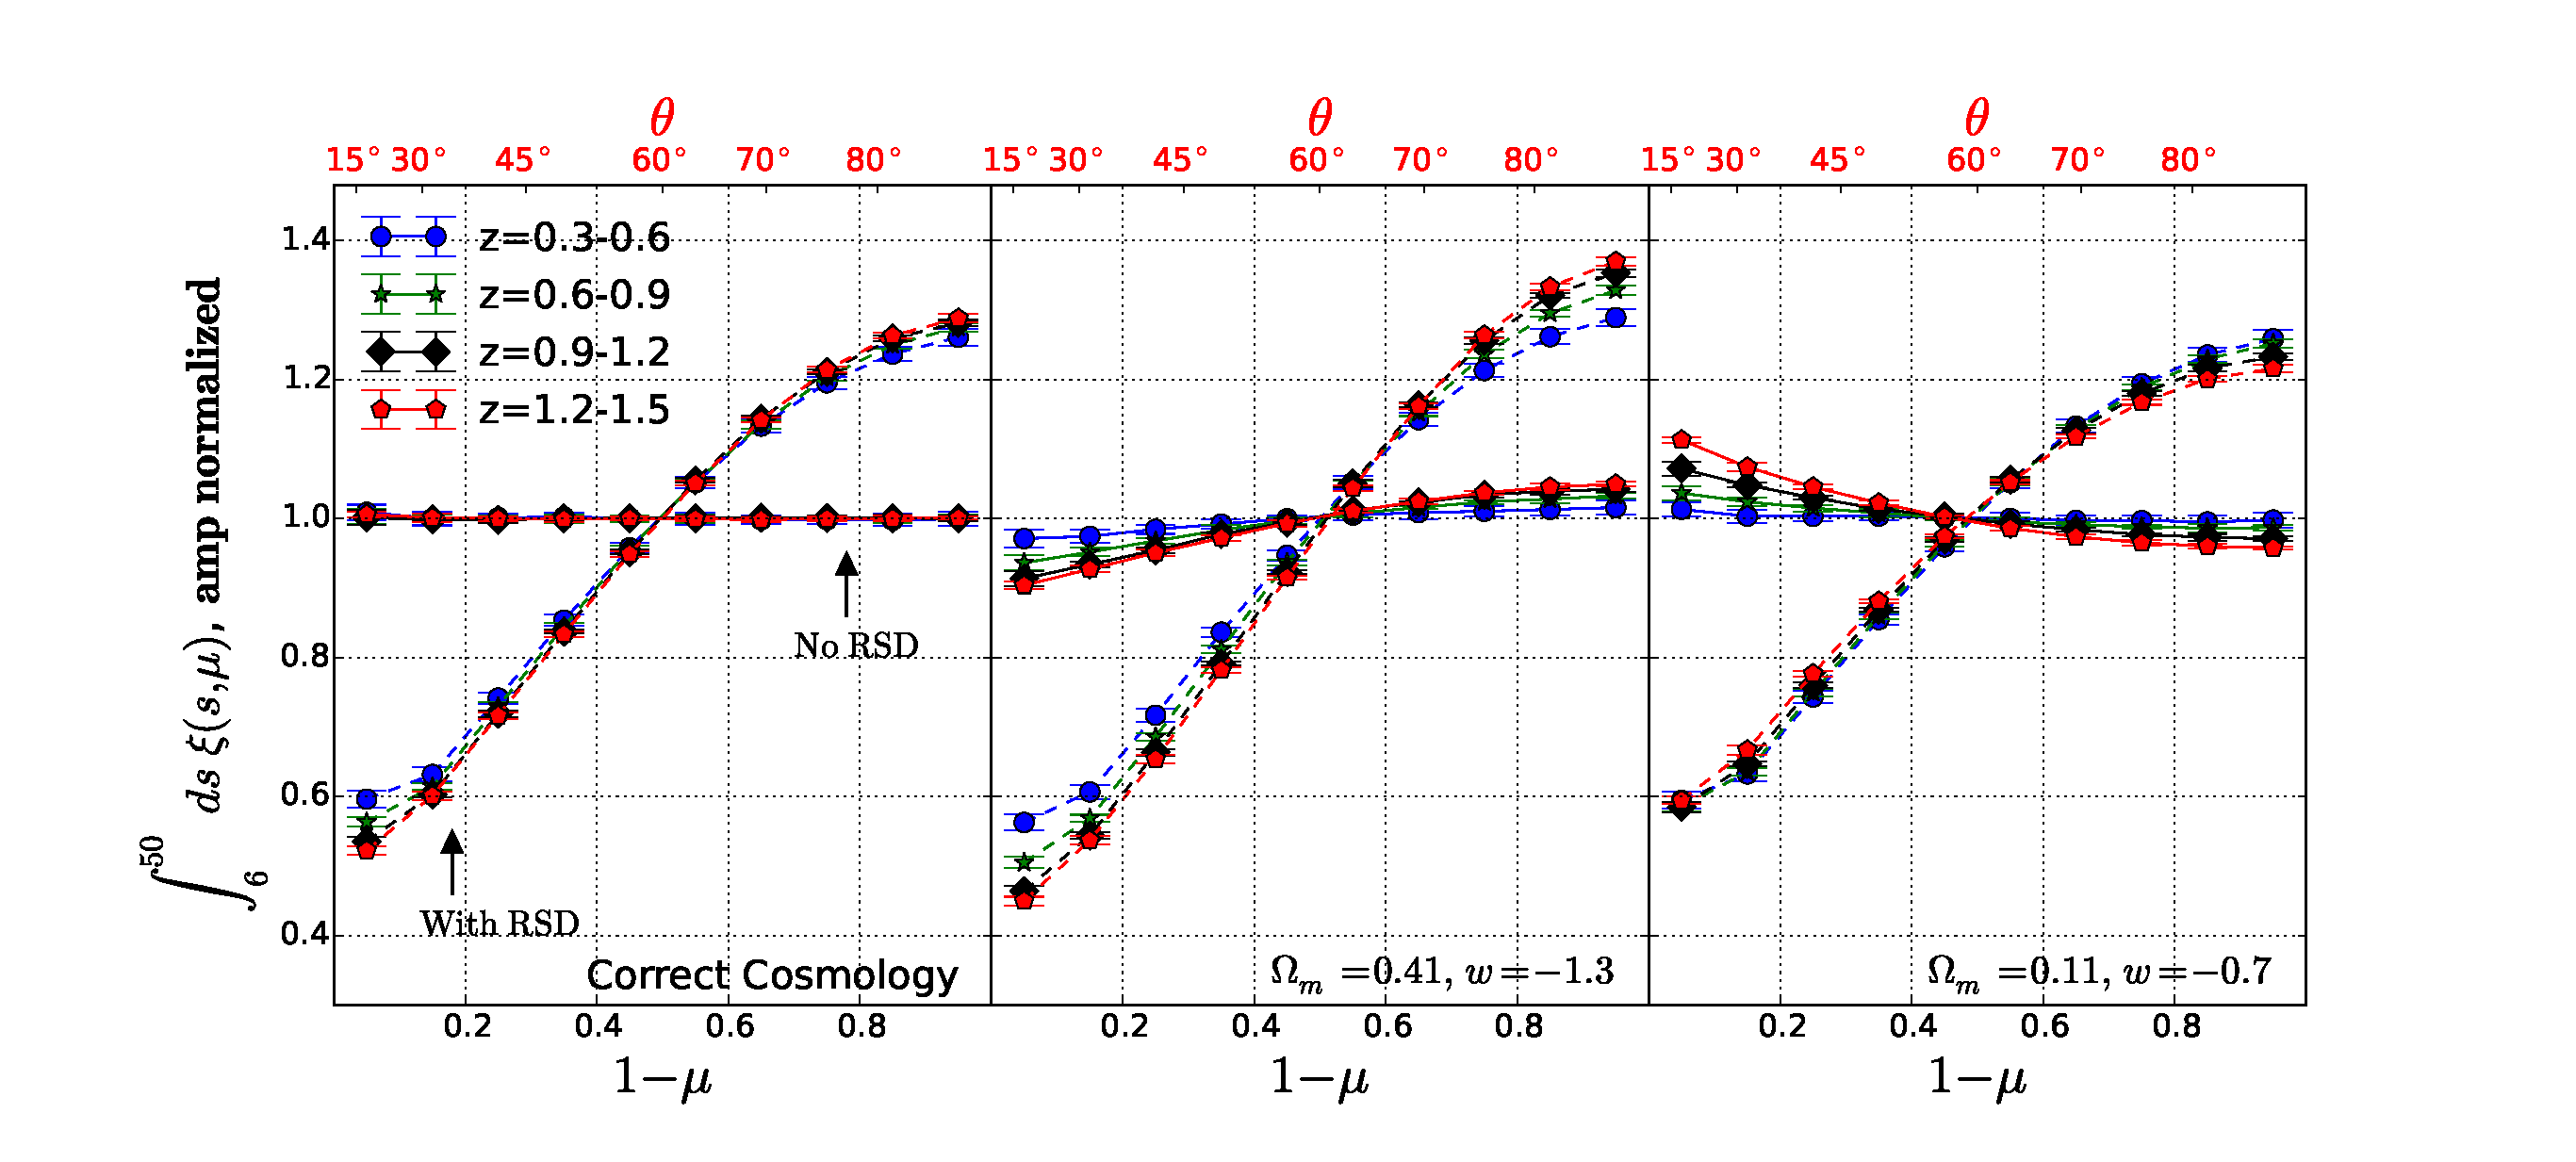
\includegraphics[height=8cm]{Tpcf--plot--Normed.eps}
%    \includegraphics[height=8cm]{smu.eps}
    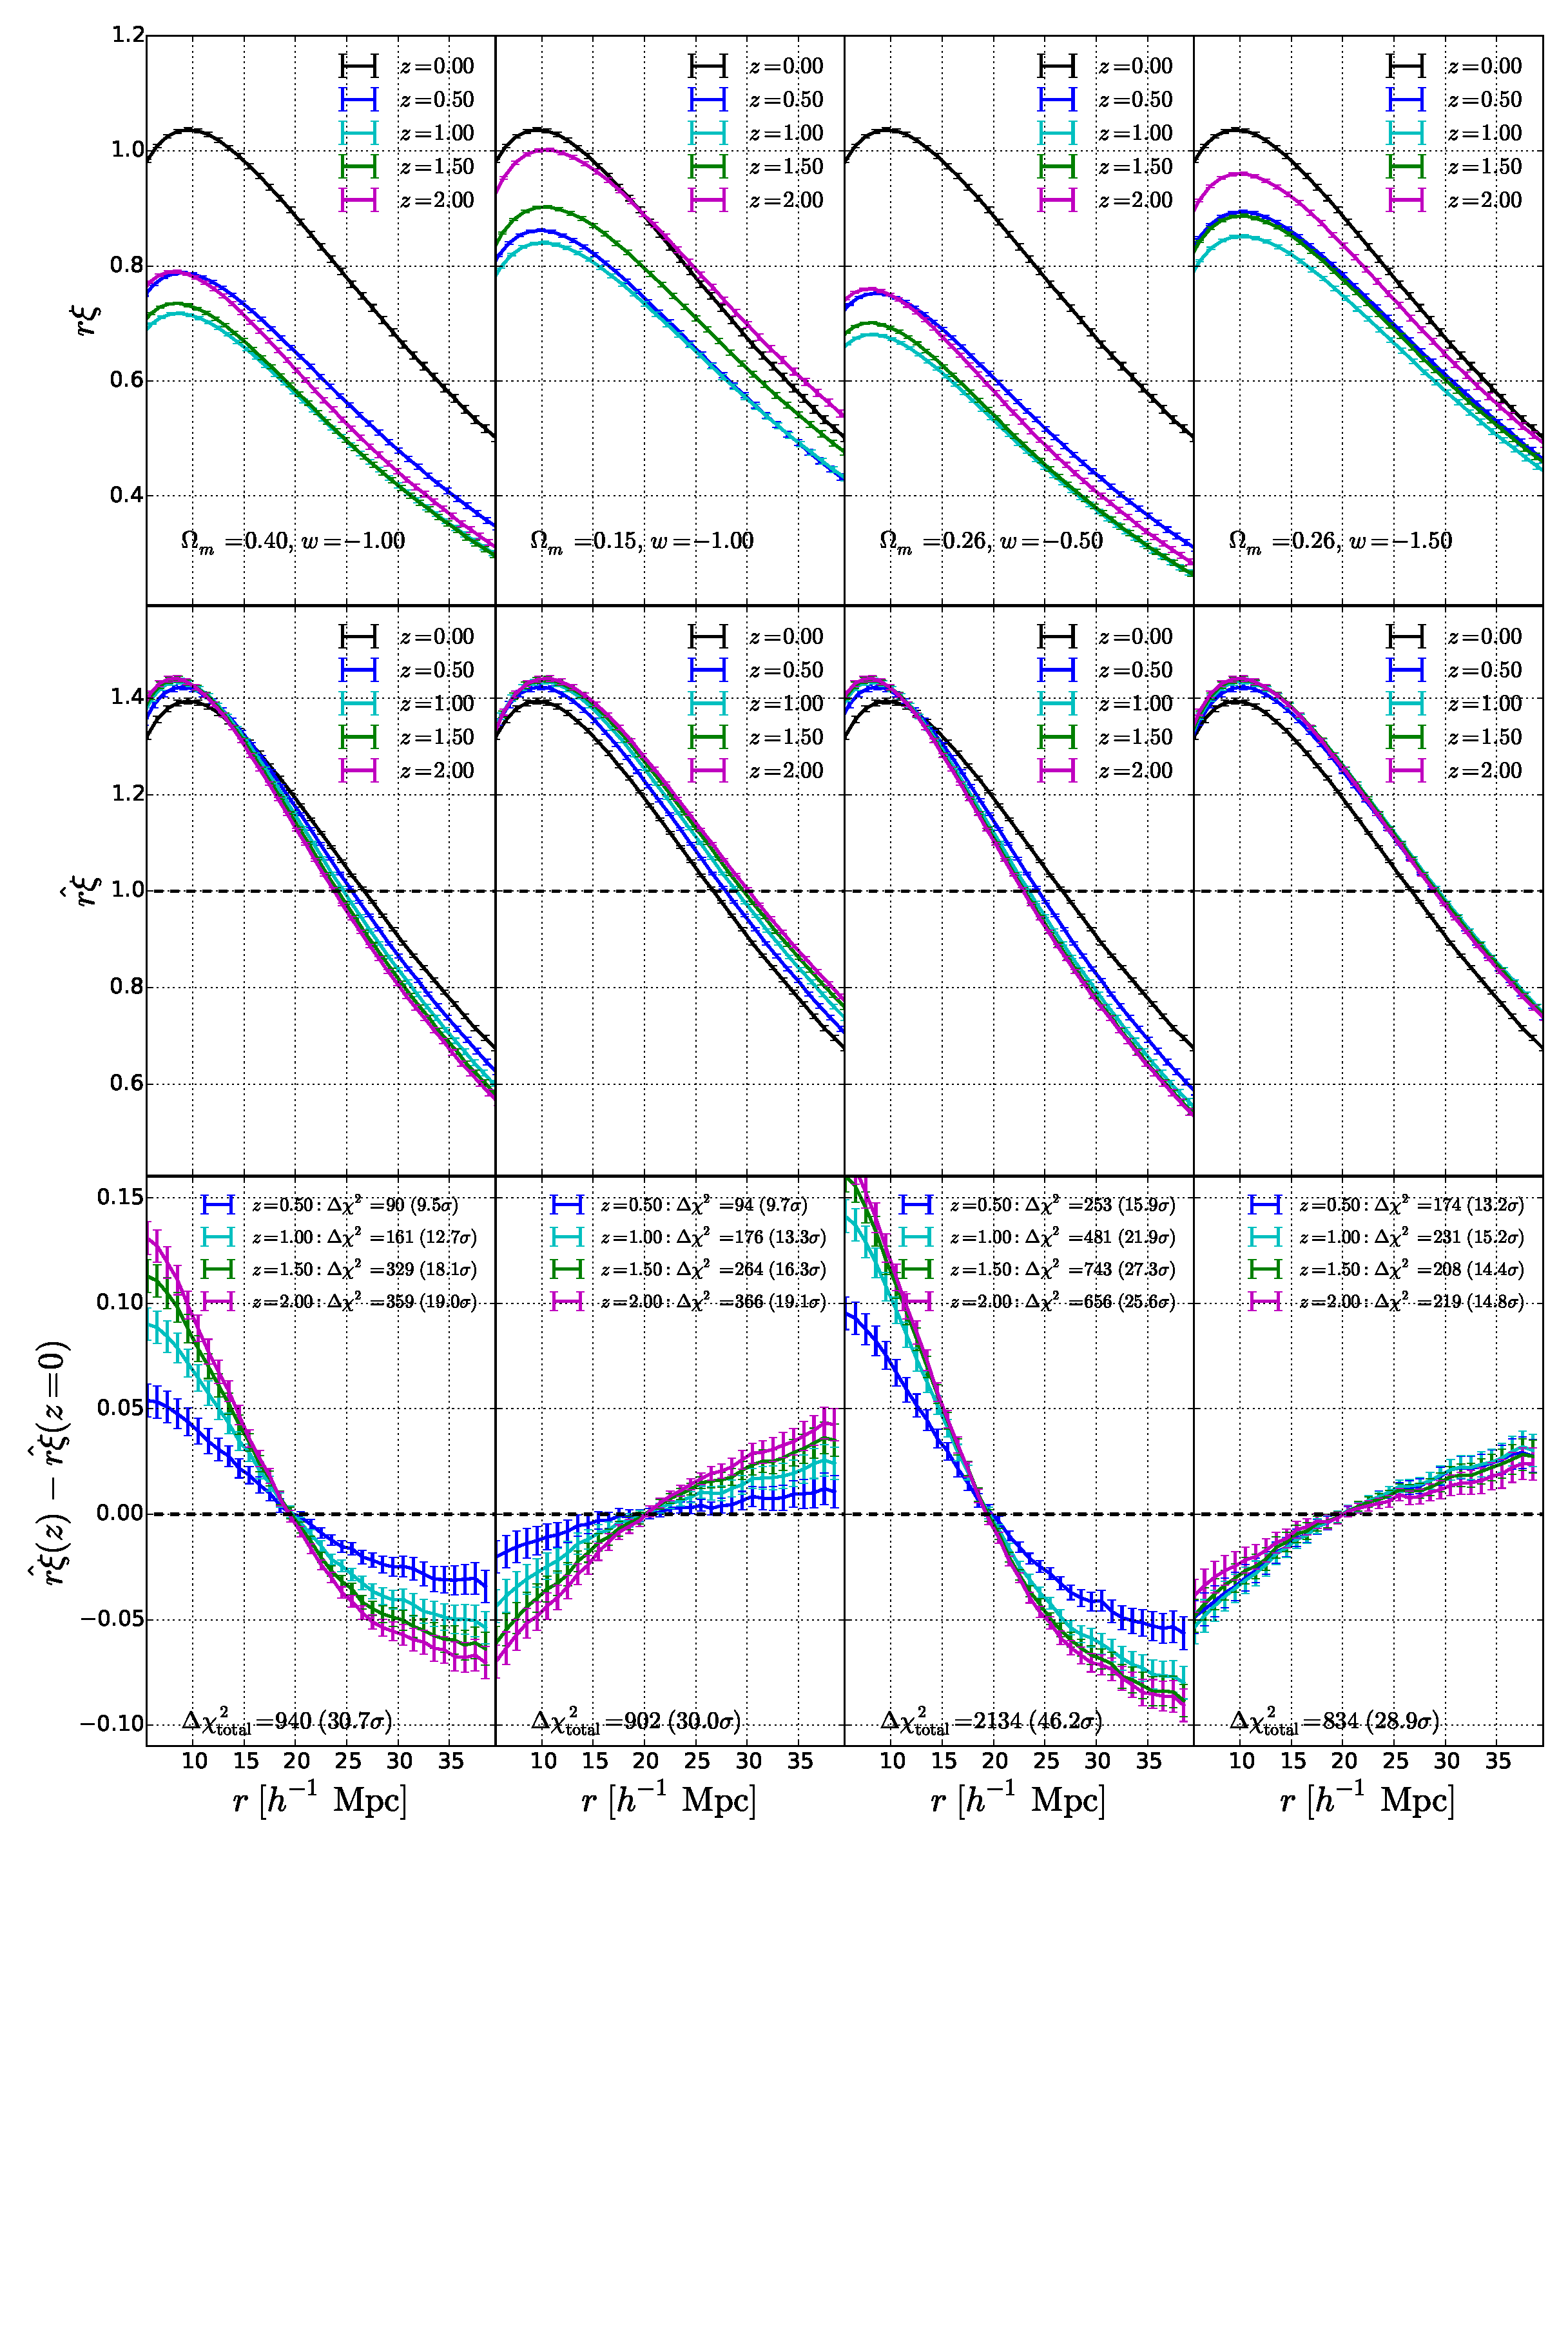
\includegraphics[width=18cm]{fig4.eps}
   }
   \caption{\label{fig_cosmo}
   2pCF in cosmologies.
   }
\end{figure*}




\section{Cosmological constraint}



We constrain $\Omega_m$ and $w$ through Bayesian analysis (\citep{Bayesian}; also see \citep{LB2002,Li2016} for details).
We assue the likelihood takes the form
\begin{equation}
 \mathcal{L} \propto \exp\left[-\frac{\chi^2}{2}\right]
\end{equation}
and scan the parameter space in $\Omega_m-w$ plane to obtain the 68.3\% and 97.4\% CL regions.
The result is displayed in Figure \ref{fig_contours}.


\begin{figure*}
   \centering{
   %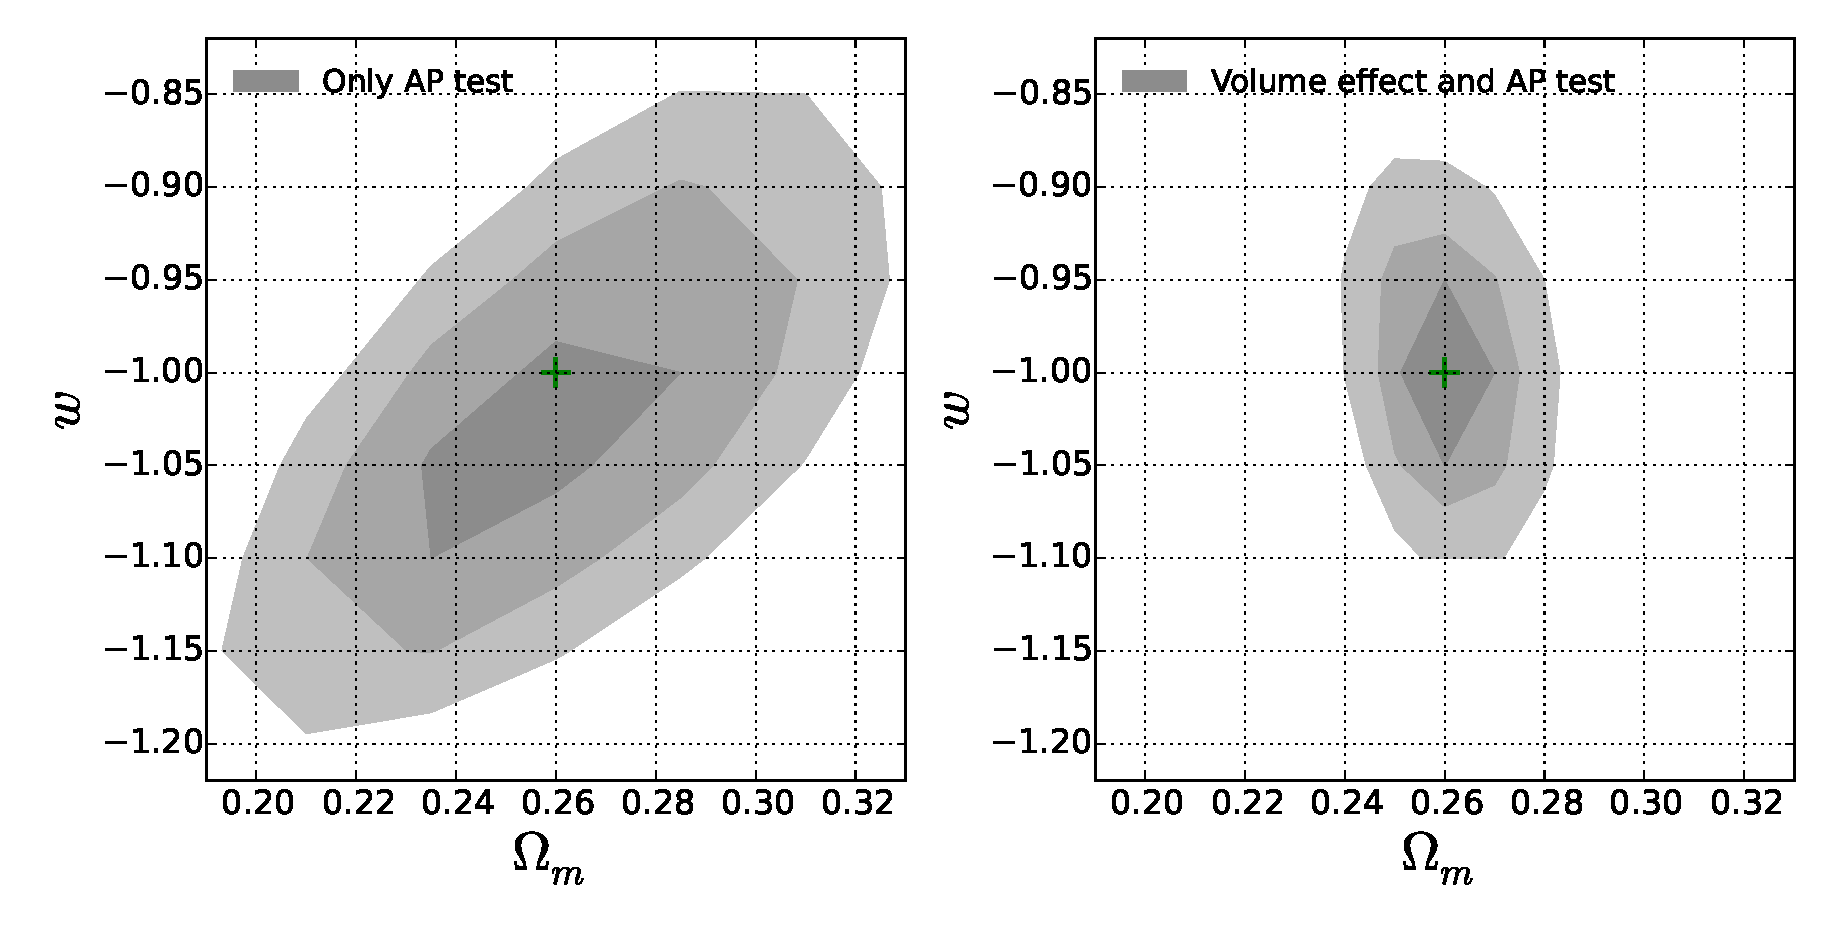
\includegraphics[width=7cm]{Tpcf--contour.eps}
   %\includegraphics[width=16cm]{Tpcf--contour-others.eps}
   %\includegraphics[width=16cm,natwidth=52,natheight=40]{fig10.eps}
   %\includegraphics[width=16cm]{fig10.eps}
   }
   \caption{\label{fig9.eps}
   Likelihood contours (68.3\%, 95.4\%) in the $\Omega_m-w$ plane from our method.
   }
\end{figure*}

We get tight constraint on the two paramters.
The 2$\sigma$ contour lies within the region $0.23<\Omega_m<0.285$, $-1.1<w<-0.9$.
The thin shape of contour means, when combining with the another observational data with different direction of degeneracy (e.g. CMB),
very tight combined constraint can be obtained.
In case of fixing one parameter at its best-fit value and infer the statistical uncertainty of the other one,
one will obtain 1$\sigma$ uncertainty of $\delta\Omega_m\approx0.002,\delta w\approx0.01$. 


\section{Concluding Remarks}



 * Can be combined with our redshift dependence of AP to full explore the geometric effects in LSS

 * *** utilizes angular 2pCF as a function of redshift. Our method is complementary to it: 1) smaller scales; 2) more bins; 3) could be less affected by RSD; ... In case of good modelling of RSD one can rely on their; in case not possible, especially on small scales, one can use ours

 * Complementary to all other LSS probes

 * Promising future



\section*{Acknowledgments}

We thank the Korea Institute for Advanced Study for providing computing resources (KIAS Center for Advanced Computation Linux Cluster System).
%We thank Seokcheon Lee and Graziano Rossi for many helpful discussions.
We would like to thank Yi Zheng for useful discussions.
This work was partially supported by the
Supercomputing Center/Korea Institute of Science and
Technology Information with supercomputing resources
including technical support (KSC-2013-G2-003).


\appendix

\

\begin{thebibliography}{}

\bibitem[Ade et al. (2015)]{Planck2015}
Ade, P.A.R., Aghanim, N., \& Arnaud, M., et al. arXiv:1502.01589

\bibitem[Alam et al.(2016)]{Alam2016}
Alam, S., Ata, M., \& Bailey, S., et al. 2016,
submitted to MNRAS (arXiv:1607.03155)

\bibitem[{{Alam} {et~al}\mbox{.}(2015{\natexlab{a}}){Alam}, {Albareti},
  {Allende Prieto}, {Anders}, {Anderson}, {Anderton}, {Andrews}, {Armengaud},
  {Aubourg}, {Bailey}, \& et~al.}]{dr12}
{Alam} S., Albareti, F.D.,\& Allende Prieto, C., {et~al.}, 2015,  ApJS, 219, 12

\bibitem[Alcock \& Paczynski(1979)]{AP1979}
Alcock, C., \& Paczynski, B. 1979, Nature, 281, 358  

%\bibitem[Anderson et al.(2012)]{2012MNRAS.427.3435A} 
%Anderson, L., Aubourg, E., Bailey, S., et al.\ 2012, MNRAS, 427, 3435

\bibitem[Anderson et al.(2013)]{Anderson2013}
Anderson, L., Aubourg, \'E., \& Bailey, S. et al. 2014, MNRAS, 441, 24  
  
%\bibitem[Bassett et al.(2002)]{Bassett2002}
%Bassett, B.A., Kunz, M., Silk, J., \& Ungarelli, C. 2002, MNRAS, 336, 1217

\bibitem[Ballinger, Peacock \& Heavens 1996]{Ballinger1996}
Ballinger, W.E., Peacock, J.A., \& Heavens, A.F. 1996, MNRAS, 282, 877  

\bibitem[Betoule et al.(2014)]{JLA}
Betoule, M., Kessler, R., \& Guy, J., et al. 2014, A\&A, 568, 32


\bibitem[Beutler et al.(2011)]{6dFGS}
Beutler, F., Blake, C., \& Colless, M., et al. 2011, MNRAS, 416, 3017

\bibitem[Beutler et al.(2013)]{Beutler2013}
Beutler, F., Saito, S., \& Seo, H.-J., et al. 2013, MNRAS, 443, 1065

\bibitem[Beutler et al.(2016)]{Beutler2016}
Beutler, F., Seo, H.-J., \& Saito, S., et al. 2016,
arXiv:1607.03150

\bibitem[Blake et al.(2011)]{Blake2011}
Blake, C., Glazebrook, K., \& Davis, T. M., 2011, MNRAS, 418, 1725  

\bibitem[Blake et al.(2013)]{WiggleZtopoloy}
Blake, C., James, J.B., \& Poole, G.B. 2013, MNRAS, 437, 2488

\bibitem[Bolton et al.(2012)]{Bolton2012}
Bolton, A.S., Schlegel, \& D.J., Aubourg E., et al. 2012, AJ, 144, 144

\bibitem[Boylan-Kolchin et al.(2008)]{B08}
Boylan-Kolchin, M., Ma, C.-P., \& Quataert, E. 2008, MNRAS, 383, 93


%\bibitem[Bueno Belloso et al. (2012)]{BB2012}
%Bueno Belloso, A., Pettinari, G.W., Meures, N., \& Percival, W.J. 2012, Phys. Rev. D, 86, 023530

%\bibitem[Chevallier \& Polarski(2001)]{CP2001}
%Chevallier, M., Polarski, D. 2001, Int. J. Mod. Phys. D, 10, 213


%\bibitem[Choi et al.(2010)]{choi 2010}
%Choi, Y.-Y., Park, C., Kim, J., Gott, J.R., 
%Weinberg, D.H., Vogeley, M.S., \& Kim, S.S. 2010, ApJS, 190, 181

\bibitem[Christensen et al.(2001)]{Bayesian}
Christensen, N., Meyer, R., Knox, L., \& Luey, B. 2001, Class. Quant. Grav., 18, 2677

%\bibitem[Chuang et al.(2013)]{Chuang2013}
%Chuang, C.-H., Prada, F., Beutler, F., et al. 2013, arXiv:1312.4889  

\bibitem[Chuang \& Wang(2012)]{ChuangWang2012}
Chuang, C.-H., \& Wang, Y. 2012, MNRAS, 426, 226  


%\bibitem[Corasaniti \& Copeland(2003)]{Corasaniti2003}
%Corasaniti, P.S., Copeland, E.J. 2003, Phys. Rev. D, 67, 063521

%eBOSS: 
%http://arxiv.org/abs/1508.04473
\bibitem[Dawson et al.(2015)]{eBOSS}
Dawson, K.S., Kneib, J.P., \& Percival, W.J., et al. 2015, accepted AJ

\bibitem[Dawson et al.(2012)]{Dawson et al. 2012}
Dawson, K.S., Schlegel, D.J., \& Ahn, C.P., et al. 2012, AJ, 145, 10

\bibitem[Efstathiou (2014)]{E14H0}
Efstathiou, G. 2014, MNRAS, 440, 1138

\bibitem[Eisenstein et al.(2011)]{Eisenstein et al. 2011}
Eisenstein, D.J.,  Weinberg, D.H., \& Agolet, E., et al. 2011, AJ, 142, 72

\bibitem[Feldman, Kaiser \& Peacock (1994)]{1994ApJ...426...23F} 
Feldman, H.A., Kaiser, N., \& Peacock, J.A.\ 1994, ApJ, 426, 23 

\bibitem[Fukugita et al. (1996)]{Fukugita1996}
Fukugita, M., Ichikawa, T., \& Gunn, J.E., et al. 1996, AJ, 111, 1748
%Publication:	
%Astronomical Journal v.111, p.1748 

%\bibitem[Gingold \& Monaghan(1977)]{GM1977}
%Gingold, R.A., \& Monaghan, J.J. 1977, MNRAS, 181, 375  

%\bibitem[Gott et al.(2009)]{gott 2009}
%Gott, J.R., Choi, Y.-Y., Park, C., \& Kim, J. 2009, ApJ, 695, L45  

%\bibitem[Gott et al.(2008)]{gott 2008}
%Gott, J.R., Hambrick, D.C., Vogeley, M.S., Kim, J., Park, C., Choi, Y.-Y.,
%Cen, R., Ostriker, J.P., \& Nagamine, K. 2008, ApJ, 675, 16  


\bibitem[Gunn et al. (1998)]{Gunn1998}	
Gunn, J.E., Carr, M., \& Rockosi, C. et al. 1998, AJ, 116, 3040

\bibitem[Gunn et al.(2006)]{Gunn et al. 2006}
Gunn, J.E., Siegmund, W.A., \& Mannery, E.J., et al. 2006, AJ, 131, 2332

\bibitem[Guzzo et al.(2008)]{Guzzo2008}
Guzzo, L., Pierleoni, M., \& Meneux, B., et al. 2008, Nature, 451, 541

\bibitem[Hartlap et al.(2006)]{Hartlap}
Hartlap J., Simon P. \& Schneider P. [astro-ph/0608064].


\bibitem[Hong et al.(2016)]{hong2016}
Hong, S.E., Park, C.,\&  Kim, J. 2016, ApJ, 823, 103

\bibitem[Jackson (1972)]{FOG}
Jackson, J., 1972, MNRAS, 156, 1

\bibitem[Jennings et al.(2011)]{Jennings2011}
Jennings, E., Baugh, C.M., \& Pascoli, S. 2011, MNRAS, 420, 1079  

%\bibitem[Jeong et al.(2014)]{Jeong2014}
%Jeong, D., Dai, L., Kamionkowski, M., \& Szalay, A.S. 2014, arXiv:1408.4648

\bibitem[Jiang et al.(2008)]{jiang2008}
Jiang, C.Y., Jing, Y. P., \& Faltenbacher, A., et al. 2008, ApJ, 675, 1095

\bibitem[Kaiser (1987)]{Kaiser1987}
Kaiser, N. 1987, MNRAS, 227, 1


\bibitem[Kim \& Park(2006)]{kim and park 2006}
Kim, J., \& Park, C. 2006, ApJ, 639, 600  

\bibitem[Kim et al.(2009)]{2009ApJ...701.1547K} 
Kim, J., Park, C., Gott, J.R., III, \& Dubinski, J.\ 2009, ApJ, 701, 1547 

\bibitem[Kim et al.(2015)]{hr4}
Kim, J., Park, C., L'Huillier, B., \& Hong, S. E. 2015, JKAS, 48, 213

\bibitem[Kim et al.(2011)]{horizonrun}
Kim, J., Park, C., Rossi, G., Lee, S.M., \& Gott, J.R. 2011, JKAS, 44, 217  

\bibitem[Kitaura et al.(2015)]{MDPATCHY}
Kitaura, F.S., Rodrı\'{i}guez-Torres, S., Chuang, C.-H., et al. arXiv:1509.06400

\bibitem[Komatsu et al.(2011)]{komatsu 2011}
Komatsu, E., Smith, K. M., \& Dunkley, J., et al. 2011, ApJS, 192, 18  

\bibitem[Lacey \& Cole(1993)]{LC93}
Lacey, C., \& Cole, S. 1993, MNRAS, 262, 627


\bibitem[Landy \& Szalay(1993)]{1993ApJ...412...64L} 
Landy, S.D., \& Szalay, A.S.\ 1993, ApJ, 412, 64 

%EUCLID:
%http://arxiv.org/abs/1110.3193
\bibitem[Laureijs et al.(2011)]{EUCLID}
Laureijs, R., Amiaux, J., \& Arduini, S., et al. 2011, arXiv:1110.3193

\bibitem[Lavaux \& Wandelt(2012)]{LavausWandelt1995}
Lavaux, G., \& Wandelt, B.D. 2012, ApJ, 754, 109  

%\bibitem[Levi et al.(2013)]{2013arXiv1308.0847L} 
%Levi, M., Bebek, C., Beers, T., et al.\ 2013, arXiv:1308.0847 

\bibitem[Lewis \& Bridle (2002)]{LB2002}
Lewis, A., \& Bridle, S. 2002, Phys. Rev. D, 66, 103511

\bibitem[L'Huillier et al.(2014)]{2014NewA...30...79L} 
L'Huillier, B., Park, C., \& Kim, J.\ 2014, New Astronomy, 30, 79 

\bibitem[Li et al.(2011)]{Li2011}
Li, M., Li, X.-D., Wang, S., \& Wang, Y. 2011, Commun. Theor. Phys., 56, 525

\bibitem[Li et al.(2014)]{Li2014}
Li, X.-D., Park, C., Forero-Romero, J., \& Kim, J. 2014, ApJ, 796, 137

\bibitem[Li et al.(2015)]{Li2015}
Li, X.-D., Park, C., Sabiu, C.G., \& Kim, J. 2015, MNRAS, 450, 807 

\bibitem[Li et al.(2016)]{Li2016}
Li, X.-D., Park, C., Sabiu, C.G., \& Kim, J. 2016, submitted to ApJ


%\bibitem[Linder(2003)]{Linder2003}
%Linder, E.V. 2003, Phys. Rev. Lett., 90, 091301

\bibitem[Linder et al.(2014)]{Linder2013}
Linder, E.V., Minji, O., Okumura, T., Sabiu, C.G., \& Song, Y.-S. 2014, Phys. Rev. D, 89, 063525  

\bibitem[L{\'o}pez-Corredoira(2014)]{2014ApJ...781...96L} 
L{\'o}pez-Corredoira, M.\ 2014, ApJ, 781, 96 

\bibitem[Marinoni \& Buzzi(2010)]{Marinoni2010}
Marinoni, C., \& Buzzi, A. 2010, Nature, 468, 539  

\bibitem[Matsubara \& Suto(1996)]{Matsubara1996}
Matsubara T., \& Suto, Y. 1996, ApJ, 470, L1  

\bibitem[McCavana et al.(2012)]{M12}
McCavana, T., Micic, M., Lewis, G. F., et al. 2012, MNRAS, 424, 361


\bibitem[Morandi \& Sun (2016)]{MS2016}
Morandi, A., \& Sun, M. arXiv:1601.03741


\bibitem[Outram et al.(2004)]{Outram2004}
Outram, P.J., Shanks, T., Boyle, B.J., Croom, S.M., Hoyle, F., Loaring, N.S., 
Miller, L., \& Smith, R.J. 2004, MNRAS, 348, 745  

%\bibitem[Parejko et al.(2013)]{Parejko2013}
%Parejko, J. K., Sunayama, T., Padmanabhan, N., et al. 2013, MNRAS, 429, 98  

\bibitem[Parejko et al.(2013)]{Parejko2013}
Parejko J.K., et al., 2013, MNRAS, 429, 98

\bibitem[Parihar et al. (2014)]{CMASSLSS2014}
Parihar, P., Vogeley, M.S., \& Gott, J.R., et al. 2014, ApJ, 796, 86

\bibitem[Park et al.(2005)]{park 2005}
Park, C., Kim, J., \& Gott, J.R. 2005, ApJ, 633, 1  

\bibitem[Park \& Kim(2010)]{topology}
Park, C., \& Kim, Y.-R. 2010, ApJL, 715, L185  

\bibitem[Park et al. (2012)]{Park2012}
Park, C., Choi, Y.-Y., Kim, J., Gott, J.R., Kim, S.S., \&
Kim, K.-S. 2012, ApJ, 759, 7

\bibitem[Park et al. (2015)]{Park2015}
Park, C., Song, H., Einasto, M., Lietzen, H., \&
Heinamaki, P. 2015, JKAS, 48, 75

\bibitem[Peebles \& Ratra(2003)]{PR2003}
Peebles, P.J.E., \& Ratra, B. 2003, Reviews of Modern Physics, 75, 559

\bibitem[Percival et al.(2014)]{Percival2014}
Percival, W.J., Ross, A.J., \& S\'{a}nchez, A.G., et al. 2014, MNRAS, 439, 2531

\bibitem[Perlmutter et al.(1999)]{Perl1999}
Perlmutter, S., Aldering, G., \& Goldhaber, G., et al. 1999, ApJ, 517, 565  

\bibitem[Press \& Shechter(1974)]{PS1974}
Press, W.H., \& Schechter, P.L. 1974, ApJ, 187, 425

\bibitem[Reid et al.(2012)]{Reid2012}
Reid, B., Samushia, L., \& White, M., et al. 2012, MNRAS, 426, 2719  

\bibitem[Reid et al.(2016)]{Reidetal:2016}
Reid, B., Ho, S., \& Padmanabhan, N., et al.  2016, MNRAS, 455, 1553

\bibitem[Riess et al.(1998)]{Riess1998}
Riess, A.G., Filippenko, A.V., \& Challis, P., et al. 1998, AJ, 116, 1009  

\bibitem[Riess et al.(2011)]{Riess2011}
Riess, A.G., Macri, L., \& Casertano, S., et al. 2011, ApJ, 730, 119
%A 3\% Solution: Determination of the Hubble Constant with the Hubble Space Telescope and Wide Field Camera

\bibitem[Ross et al.(2012)]{2012MNRAS.424..564R} 
Ross, A.J., Percival, W.J., \& S{\'a}nchez, A.G. et al.\ 2012, MNRAS, 424, 564 

\bibitem[Ross et al.(2015)]{MGS}
Ross, A.J., Samushia, L., \& Howlett, C., et al. 2015, MNRAS, 449, 835

\bibitem[Ryden(1995)]{Ryden1995}
Ryden, B.S. 1995, ApJ, 452, 25  

%\bibitem[Samushia et al.(2014)]{Samushia2014}
%Samushia, L., Reid, B. A., White, M., et al. 2014, MNRAS, 439, 3504  

%\bibitem[Sanchez et al.(2013)]{Sanchez2013}
%Sanchez, A. G., Kazin, E. A., Beutler, F., et al. 2013, MNRAS, 433, 1202  

%\bibitem[Sutter et al.(2014)]{Sutter2014}
%Sutter, P.M., Pisani, A., Wandelt, B.D., \& Weinberg, D.H. 2014, MNRAS, 443, 2983


\bibitem[Sanchez et al.(2016)]{Sanchez2016}
Sanchez, A. G., Scoccimarro, R., \& Crocce, M., et al.
arXiv:1607.03147

\bibitem[Schlafly et al.(2010)]{Schlafly2010}
Schlafly E.F., Finkbeiner D.P., Schlegel D.J., et al. 2010, ApJ, 725, 1175

\bibitem[Schlafly \& Finkbeiner(2011)]{SF2011}
Schlafly E.F., \& Finkbeiner D.P. 2011, ApJ, 737, 103


%DESI:
%http://arxiv.org/abs/1106.1706
\bibitem[Schlegel et al.(2011)]{DESI}
Schlegel, D., Abdalla, F., \& Abraham, T., et al. 2011, arXiv:1106.1706

\bibitem[Smee et al.(2013)]{Smee2013}
Smee, S.A., Gunn, J.E., \& Uomoto, A., et al. 2013, AJ, 146, 32

\bibitem[Song et al.(2014)]{2014arXiv1407.2257S} 
Song, Y.S., Sabiu, C.G., 
Okumura, T., Oh, M., \& Linder, E.V.\ 2014, JCAP, 12, 005 

\bibitem[Speare et al. (2015)]{Speare2015}
Speare, R., Gott, J.R., Kim, J., \& Park, C.
2015, ApJ, 799, 176

%\bibitem[Tojeiro \& Percival(2011)]{Tojeiro2011}
%Tojeiro R., \& Percivial W.J. 2011, MNRAS, 417, 1114  

%\bibitem[Tojeiro et al.(2012)]{Tojeiro2012}
%Tojeiro, R., Percival, W. J., Wake, D. A., et al. 2012, MNRAS, 424, 136 

\bibitem[Viana \& Liddle(1996)]{VL1996}
Viana, P.T.P., \& Liddle, A.R. 1996, MNRAS, 281, 323

\bibitem[Villalobos et al.(2013)]{V13}
Villalobos, \'{A}., ́De Lucia, G., Weinmann, S.M., Borgani, S., \& Murante, G. 2013, MNRAS, 433, L49


\bibitem[Weinberg (1989)]{SW1989}
Weinberg, S. 1989, Reviews of Modern Physics, 61, 1

\bibitem[White (2011)]{White2011}
White M., et al. 2011, ApJ, 728, 126

\bibitem[York et al.(2000)]{York et al. 2000}
York, D.G., Adelman, J., \& Anderson, J.E., et al. 2000, AJ, 120, 1579

\bibitem[Zehavi et al.(2011)]{zehavi2011}
Zehavi, I., Zheng, Z., \& Weinberg, D.H., et al. 2011, ApJ, 736, 59




\end{thebibliography}


\end{document}
